\chapter{多目标优化}
\label{chap:multi-objective-optimization}

一个方案要同时看成本和误差。方案甲花$1$万元，误差是$8$个百分点；方案乙花$6$万元，误差是$1$个百分点。甲便宜，乙准确，两个数字都要小，却没有哪一个同时更小。前面各章的比较都落在一条数轴上，这里的比较落在一个平面上，“谁更好”这个问题第一次没有现成的答案。

常见的做法是把两个目标加起来再求解。这样做当然能得到一个数，但成本和误差的单位不同，加法里藏着一个没有说出口的汇率。换一个单位，或者换一个汇率，答案就可能换成另一个方案。所以本章要问的是：在没有汇率之前，哪些比较是站得住的？有了某种偏好之后，怎样把它写成单目标问题？需要给决策者看一整组候选的时候，怎样把这组候选算出来，又怎样判断它算得好不好？

本章先建立不依赖偏好的比较关系，得到一组互不支配的方案。然后讨论三种写出偏好的办法，比较它们各能到达哪些方案。接着转到局部信息，研究什么时候还存在让所有目标一起下降的小步，并由此构造一个不预设偏好的迭代。最后讨论怎样组织多次求解或一个种群来近似整条前沿，以及未知真实前沿时能够报告哪些量。

全章反复使用几个小例子：六个有限候选、两个二次函数，以及两条非凸的前沿。每种方法都放到这几个例子上算一遍，看它到得了哪里、到不了哪里。

\section{多目标问题}
\label{sec:moo-problem}

目标从一个数变成一组数之后，“更好”和“最优”还能怎样定义？本节先把问题写出来，再找出不需要任何偏好就能成立的比较，最后说明目标的单位会影响哪些判断。

\paragraph{问题的形式}
在同一个可行集上，同时要求$m$个目标都尽量小，这样的问题称为\term{多目标优化}（multi-objective optimization）：
\begin{equation}
 \min_{\bm{x}\in\bm{C}}\ \bm{f}(\bm{x})=\bigl(f_1(\bm{x}),\ldots,f_m(\bm{x})\bigr).
 \label{eq:moo-problem}
\end{equation}
本章的$m$始终表示目标个数。需要写约束函数时，第~\ref{sec:moo-feasible-direction}节会另外安排下标。这里的“$\min$”暂时只是一个愿望，它的含义正是本节要确定的。

问题涉及两个空间。变量$\bm{x}$所在的$\mathbb{R}^n$称为\term{决策空间}（decision space），目标向量所在的$\mathbb{R}^m$称为\term{目标空间}（objective space）。可行集在$\bm{f}$下的像
\begin{equation}
 \bm{Y}=\bm{f}(\bm{C})=\{\bm{f}(\bm{x}):\bm{x}\in\bm{C}\}
 \label{eq:moo-reachable}
\end{equation}
是所有能够实现的目标向量，称为\term{可达目标集}（attainable objective set）。决定方案好坏的比较发生在$\bm{Y}$里，而真正要交出去的方案在$\bm{C}$里。

\paragraph{两个贯穿全章的例子}
第一个例子是有限个候选。六个方案的成本$f_1$（万元）和误差$f_2$（百分点）如下，数据是教学用的假设：
\begin{equation}
 \begin{gathered}
  A=(1,8),\quad B=(2,5),\quad C=(4,4),\\
  D=(6,1),\quad E=(5,6),\quad F=(7,1).
 \end{gathered}
 \label{eq:moo-candidates}
\end{equation}
这里决策空间就是六个方案的名字，目标空间是平面，$\bm{Y}$由六个点组成。

第二个例子是连续的。取$\bm{C}=\mathbb{R}^2$，两个目标分别希望靠近两个不同的点：
\begin{equation}
 f_1(\bm{x})=\frac12\lVert\bm{x}-\bm{a}\rVert_2^2,\qquad
 f_2(\bm{x})=\frac12\lVert\bm{x}-\bm{b}\rVert_2^2,
 \label{eq:moo-iso}
\end{equation}
其中$\bm{a}=(1,0)$，$\bm{b}=(0,1)$。想象两个仓库分别在$\bm{a}$和$\bm{b}$，要选一个地点，离两个仓库都要近。

图~\ref{fig:moo-two-spaces}把这个映射画了出来。左边是决策平面，右边是目标平面，浅蓝色区域是$\bm{Y}$。点$\bm{p}=(1,1)$与$\bm{p}'=(0,0)$关于直线$x_1+x_2=1$对称，到两个仓库的距离分别相同，所以落到目标平面上的同一点$(1/2,1/2)$。一个目标向量可以对应多个方案，这正是不能只在目标空间里回答“选哪个方案”的原因。

\begin{BookInlineFigure}
  \centering
  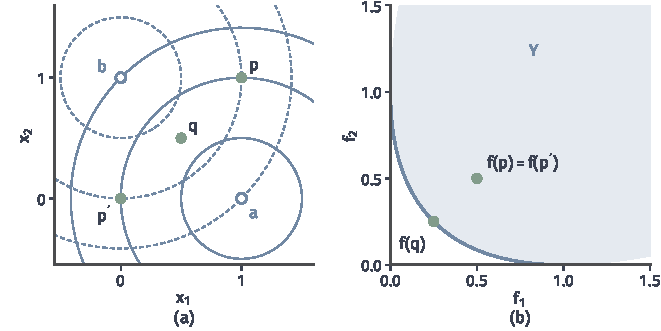
\includegraphics[width=112mm]{figures/05-optimization/07-multiple-criteria-and-nested-optimization/matplotlib/moo-two-spaces/figure.pdf}
  \caption{式~\eqref{eq:moo-iso}的决策空间与目标空间。(a)实线圆是$f_1$的等高线，虚线圆是$f_2$的等高线，绿点是三个方案。(b)浅蓝区域是可达目标集$\bm{Y}$，蓝线是它的左下边界。$\bm{p}$与$\bm{p}'$对称，映到同一个目标向量；$\bm{q}=(1/2,1/2)$的目标向量是$(1/4,1/4)$，两个分量都更小。}
  \label{fig:moo-two-spaces}
\end{BookInlineFigure}

\paragraph{为什么没有唯一的最小}
单目标问题中，任意两个实数都能比较大小，所以最小值的定义不会有歧义。向量没有这样的全序。$A=(1,8)$与$D=(6,1)$相比，成本是$A$小，误差是$D$小。两个分量的优劣方向相反，要断定谁更好，必须先说清一万元相当于多少个百分点的误差，而题目没有给出这个信息。

因此不能指望从式~\eqref{eq:moo-problem}直接得到一个点。接下来只保留不需要换算就能下的判断。

\subsection{支配关系}
\label{sec:moo-dominance}

不引入任何偏好，还能确定哪些比较？回到式~\eqref{eq:moo-candidates}，$B=(2,5)$与$E=(5,6)$相比，$B$更便宜，误差也更小。无论决策者多看重成本或多看重误差，只要两项都是越小越好，就没有理由选$E$。把这种“全面不差”写成定义。

\begin{definition}[支配]
\label{def:moo-dominance}
设$\bm{u},\bm{v}\in\bm{C}$。若
\begin{equation}
 f_i(\bm{u})\leq f_i(\bm{v})\quad\text{对所有}\ i=1,\ldots,m,
 \label{eq:moo-dom-weak}
\end{equation}
并且至少有一个$i$使$f_i(\bm{u})<f_i(\bm{v})$，就说$\bm{u}$\term{支配}（dominate）$\bm{v}$。
\end{definition}

式~\eqref{eq:moo-dom-weak}说的是“每一项都不差”，后半句说的是“至少有一项确实更好”。后半句不能省：没有它，两个目标向量相同的方案就会互相支配，而它们之间其实没有优劣。

\paragraph{用左下区域检查}
在目标平面上，支配关系可以一眼看出。以一点$\bm{y}$为角画出它的左下方区域和右上方区域，落在左下方的点支配$\bm{y}$，落在右上方的点被$\bm{y}$支配。图~\ref{fig:moo-dominance}(a)以$B$为例，平面被两条虚线分成四块。左上和右下两块中的点一个分量比$B$小，另一个分量比$B$大，这两块就是\textbf{不可比}的区域。

\begin{BookInlineFigure}
  \centering
  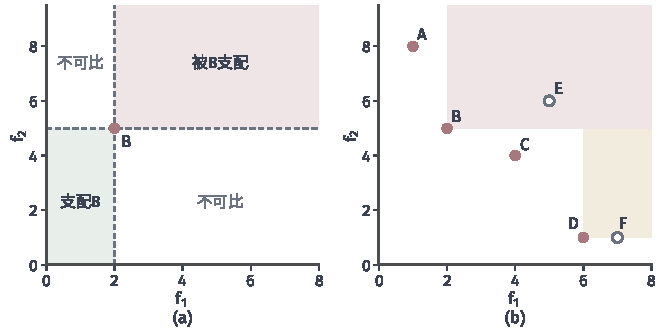
\includegraphics[width=112mm]{figures/05-optimization/07-multiple-criteria-and-nested-optimization/matplotlib/moo-dominance/figure.pdf}
  \caption{目标平面上的支配关系，数据为式~\eqref{eq:moo-candidates}。(a)以$B$为角分出的四块区域。(b)红点是不被任何候选支配的方案，空心点是被支配的方案。粉色是被$B$支配的区域，$E$在其中；浅黄是被$D$支配的区域，$F$在它的下边界上。}
  \label{fig:moo-dominance}
\end{BookInlineFigure}

下面逐对检查图~\ref{fig:moo-dominance}(b)中的六个点。$E=(5,6)$被$B$支配，也被$C=(4,4)$支配。$F=(7,1)$与$D=(6,1)$误差相同，$D$更便宜，所以$D$支配$F$。其余的$A,B,C,D$按成本从小到大排，误差依次是$8,5,4,1$，严格下降，任何两个都是一项更好、一项更差，互不支配。

支配是一种偏序：一个点不支配自己，支配关系可以传递，但并非任何两点都可比。可比的部分是确定的判断，不可比的部分要等偏好来决定。

\subsection{Pareto最优}
\label{sec:moo-pareto}

既然只有部分方案之间能比较，“最优”就只能退一步定义：没有被其他方案全面超过。这一小节给出这个定义及其两种变形，并把它们落到两个例子上。

\begin{definition}[Pareto最优]
\label{def:moo-pareto}
设$\bar{\bm{x}}\in\bm{C}$。
\begin{enumerate}
 \item 若不存在$\bm{x}\in\bm{C}$支配$\bar{\bm{x}}$，称$\bar{\bm{x}}$为\term{Pareto最优}（Pareto optimal）点。
 \item 若不存在$\bm{x}\in\bm{C}$使$f_i(\bm{x})<f_i(\bar{\bm{x}})$对所有$i$成立，称$\bar{\bm{x}}$为\term{弱Pareto最优}（weakly Pareto optimal）点。
 \item 若存在$r>0$，使上述条件在$\bm{C}$与$\bar{\bm{x}}$的$r$邻域的交集上成立，相应地称为\term{局部Pareto最优}（locally Pareto optimal）点或局部弱Pareto最优点。
\end{enumerate}
全体Pareto最优点组成的集合称为\term{Pareto解集}（Pareto set），记为$\bm{X}_{\mathrm{P}}$；它在$\bm{f}$下的像$\bm{Y}_{\mathrm{P}}=\bm{f}(\bm{X}_{\mathrm{P}})$称为\term{Pareto前沿}（Pareto front）。
\end{definition}

解集在决策空间，前沿在目标空间，二者不是同一个东西。多个方案可以对应前沿上的同一点，所以由前沿反推方案时还要保留决策变量。

未加“局部”二字的Pareto最优指全局版本，比较对象是全部可行点。全局Pareto最优点必定是局部Pareto最优点，因为比较的范围缩小了。Pareto最优点必定是弱Pareto最优点，因为所有分量都严格更小的点一定支配它。

\paragraph{有限例}
在式~\eqref{eq:moo-candidates}中，$A,B,C,D$都不被支配，都是Pareto最优点。$E$被$B$支配，且$B$的两个分量都严格小于$E$，所以$E$连弱Pareto最优点也不是。

$F=(7,1)$被$D$支配，因此不是Pareto最优点。可是要两个分量都严格小于$F$，误差必须小于$1$，而六个方案中没有这样的。所以$F$是弱Pareto最优点。弱Pareto最优这个说法宽松，正是因为它放过了“一项持平、另一项更差”的方案。

\paragraph{弱Pareto点在目标平面上的样子}
图~\ref{fig:moo-weak-pareto}中可达集合的边界有三段。红色曲线段上的点都是Pareto最优的。左侧的竖直边上，$\bm{y}$的左下方开象限（绿色）里没有可达点，所以$\bm{y}$是弱Pareto最优的；但沿着竖直边往下走到$\bm{y}'$，成本不变而误差变小，$\bm{y}'$支配$\bm{y}$。底部的水平边同理，$\bm{z}'$支配$\bm{z}$。

\begin{BookInlineFigure}
  \centering
  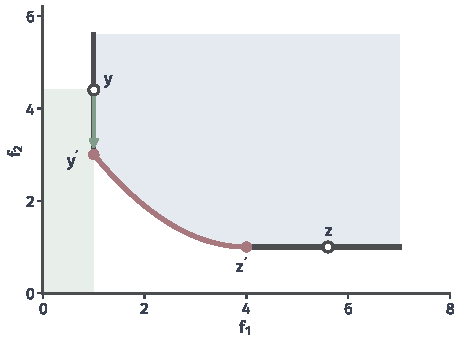
\includegraphics[width=78mm]{figures/05-optimization/07-multiple-criteria-and-nested-optimization/matplotlib/moo-weak-pareto/figure.pdf}
  \caption{弱Pareto最优点的位置。浅蓝区域是可达目标集，红色曲线是Pareto前沿，深灰粗线是只有弱Pareto性质的竖直边和水平边。绿色是$\bm{y}$的左下方开象限，其中没有可达点。绿色箭头指向支配$\bm{y}$的点$\bm{y}'$。}
  \label{fig:moo-weak-pareto}
\end{BookInlineFigure}

\paragraph{连续例：解集是一条线段}
现在求式~\eqref{eq:moo-iso}的Pareto解集。选坐标把几何关系拆开：把点写成沿$\bm{a}\to\bm{b}$的位置$s$与到连线的带符号距离$r$，
\[
 \bm{x}=\bm{a}+s(\bm{b}-\bm{a})+r\bm{e},\qquad \bm{e}=\tfrac{1}{\sqrt2}(1,1).
\]
由于$\bm{e}$是与$\bm{b}-\bm{a}$垂直的单位向量，且$\lVert\bm{b}-\bm{a}\rVert_2^2=2$，由勾股定理得到
\begin{equation}
 f_1=s^2+\tfrac12r^2,\qquad f_2=(1-s)^2+\tfrac12r^2.
 \label{eq:moo-iso-coords}
\end{equation}

式~\eqref{eq:moo-iso-coords}说明，三种情形下都能找到严格更好的点。若$r\neq0$，把$r$改为$0$，两个目标都严格减小。若$r=0$而$s<0$，把$s$改为$0$，$f_1$从$s^2$减为$0$，$f_2$从$(1-s)^2$减为$1$，两项都严格减小。$s>1$时对称。

所以Pareto最优点只可能在线段$s\in[0,1]$，$r=0$上。还要确认线段上的点确实不被支配。设$\bm{y}$支配线段上参数为$s$的点，按上面的做法把$\bm{y}$拉回线段得到参数$s'$，目标不增，于是$\bm{f}$在$s'$处的值逐项不大于在$s$处的值。

线段上$f_1=s^2$严格递增，$f_2=(1-s)^2$严格递减，两项同时不大于只能发生在$s'=s$。这样拉回前后目标向量相等，$\bm{y}$与原点目标相同，与“支配”矛盾。于是
\begin{equation}
 \bm{X}_{\mathrm{P}}=\{(1-s,s):0\leq s\leq1\},\qquad
 \bm{Y}_{\mathrm{P}}=\{(s^2,(1-s)^2):0\leq s\leq1\}.
 \label{eq:moo-iso-front}
\end{equation}

图~\ref{fig:moo-pareto-set-front}画出这一结果。线段外的点$\bm{p}=(1,1)$对应目标向量$(1/2,1/2)$，沿箭头移到$\bm{q}$后目标变成$(1/4,1/4)$，两项都减半。线段内部沿着线段移动，则是拿$f_1$换$f_2$，这种交换就是\term{取舍}（trade-off）的含义。

\begin{BookInlineFigure}
  \centering
  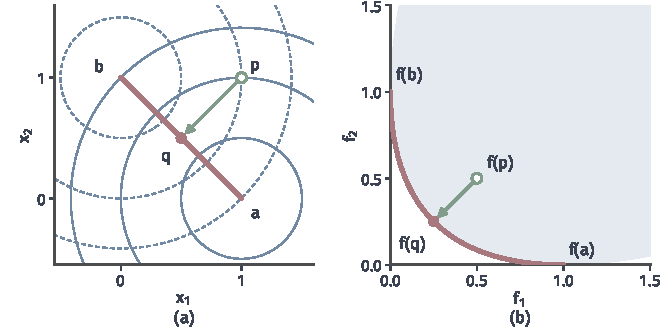
\includegraphics[width=112mm]{figures/05-optimization/07-multiple-criteria-and-nested-optimization/matplotlib/moo-pareto-set-front/figure.pdf}
  \caption{式~\eqref{eq:moo-iso}的Pareto解集与Pareto前沿。(a)决策平面上红色线段是解集，绿色箭头把线段外的点$\bm{p}$移到$\bm{q}$。(b)目标平面上浅蓝区域是可达目标集，红色曲线是前沿$(s^2,(1-s)^2)$；同一步移动使$\bm{f}(\bm{p})$沿箭头落到前沿上的$\bm{f}(\bm{q})$。}
  \label{fig:moo-pareto-set-front}
\end{BookInlineFigure}

\paragraph{局部版本与存在性}
局部Pareto最优只和附近的方案比。取一个变量$x\in[0,4]$，令
\begin{equation}
 f_1(x)=x,\qquad f_2(x)=(x-1)^2(x-3)^2+0.4x.
 \label{eq:moo-local}
\end{equation}
由于$f_1$随$x$增大，$x$越大的方案越贵，所以一个方案不被支配，要求所有更便宜的方案的误差都更大。

图~\ref{fig:moo-local-pareto}是这条曲线。$f_2$的第一个极小点约在$x\approx0.953$，记对应点为$\bm{P}$，$[0,0.953]$上的$f_2$严格下降，这一段是全局Pareto最优的（红色）。第二个极小点约在$x\approx2.946$，记对应点为$\bm{Q}$，通往$\bm{Q}$的紫色下降段上，近处更便宜的方案误差更大，近处更贵的方案误差更小，互不支配，所以这一段局部Pareto最优。

但$\bm{Q}$的两个分量约为$(2.946,1.189)$，$\bm{P}$的两个分量约为$(0.953,0.390)$，都更小，$\bm{P}$支配$\bm{Q}$。这和单目标问题中局部最小点与全局最小点的差别是一回事，只是这里比较的是向量。

\begin{BookInlineFigure}
  \centering
  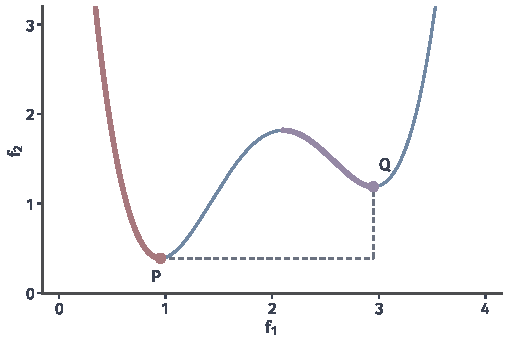
\includegraphics[width=86mm]{figures/05-optimization/07-multiple-criteria-and-nested-optimization/matplotlib/moo-local-pareto/figure.pdf}
  \caption{式~\eqref{eq:moo-local}在目标平面上的曲线。红色段全局Pareto最优，紫色段只局部Pareto最优，蓝色段的点在近处已被支配。虚线标出$\bm{P}$支配$\bm{Q}$的两个分量差。}
  \label{fig:moo-local-pareto}
\end{BookInlineFigure}

Pareto最优点也不是总存在的。取$\bm{C}=(0,1]$，$f_1(x)=f_2(x)=x$，任意$x$都被$x/2$支配，解集是空集。这和单目标问题中最小点不存在是同一种情形，第~\ref{sec:moo-scalarization}节会给出一个保证存在的条件。

\subsection{目标尺度}
\label{sec:moo-scale}

单位是人为选定的。把成本从万元换成千元，数字扩大十倍，这时哪些结论不变，哪些结论会变？

\paragraph{支配关系不受影响}
若把每个目标换成$\varphi_i(f_i)$，其中$\varphi_i$严格递增，那么$f_i(\bm{u})\leq f_i(\bm{v})$与$\varphi_i(f_i(\bm{u}))\leq\varphi_i(f_i(\bm{v}))$等价，严格不等号也一样。所以支配关系、Pareto解集、弱Pareto解集都不变。换单位是$\varphi_i(y)=cy$，$c>0$，自然在其中。

\paragraph{固定权重的加权目标会变}
把两个目标按固定权重相加，比如权重取$(0.6,0.4)$，得到一个分数，分数最低的方案胜出。以万元为单位，四个Pareto方案的分数是
\[
 A:\ 3.8,\qquad B:\ 3.2,\qquad C:\ 4,\qquad D:\ 4,
\]
所以选$B$。把成本改用千元表示，$f_1$乘以$10$，权重不变，分数变成
\[
 A:\ 9.2,\qquad B:\ 14,\qquad C:\ 25.6,\qquad D:\ 36.4,
\]
这回选$A$。方案本身什么也没变，变的只是记账单位，见图~\ref{fig:moo-scale-weight}。

\begin{BookInlineFigure}
  \centering
  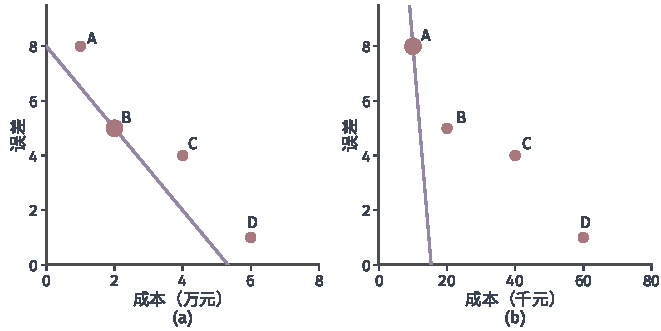
\includegraphics[width=112mm]{figures/05-optimization/07-multiple-criteria-and-nested-optimization/matplotlib/moo-scale-weight/figure.pdf}
  \caption{换单位改变加权和的选择，权重固定为$(0.6,0.4)$。紫线是经过分数最低方案的等分数线，大圆点是被选中的方案。(a)成本以万元计，选中$B$。(b)成本以千元计，选中$A$。四个点的相对位置在两图中按横轴比例对应，支配关系没有变化。}
  \label{fig:moo-scale-weight}
\end{BookInlineFigure}

\paragraph{基于距离的比较也会变}
另一种常见做法是计算到\term{理想点}（ideal point）的距离。理想点的每个分量是该目标单独能达到的最小值，这里是$(1,1)$。以万元为单位，四个方案到理想点的欧氏距离约为
\[
 A:\ 7,\qquad B:\ 4.12,\qquad C:\ 4.24,\qquad D:\ 5,
\]
$B$最近。改用千元后，理想点变为$(10,1)$，距离约为
\[
 A:\ 7,\qquad B:\ 10.77,\qquad C:\ 30.15,\qquad D:\ 50,
\]
$A$最近。距离把两个分量的差放在一起平方，单位大的分量就占了主导。

\paragraph{归一化及其参考范围}
为消除单位，常把每个目标按某个参考范围线性缩放到$[0,1]$。取目标$i$的下参考值$l_i$和上参考值$u_i$，$u_i>l_i$，令
\begin{equation}
 \tilde{f}_i=\frac{f_i-l_i}{u_i-l_i}.
 \label{eq:moo-normalize}
\end{equation}
下参考值常取理想点。上参考值常取Pareto方案中各目标的最大值，这样的点称为\term{最差点}（nadir point）。

以$A,B,C,D$的范围$l=(1,1)$，$u=(6,8)$归一化，四点变成
\[
 A:\ (0,1),\quad B:\ (0.2,0.571),\quad C:\ (0.6,0.429),\quad D:\ (1,0).
\]
到原点的距离依次约为$1$，$0.605$，$0.737$，$1$，选$B$。这一结果不再受万元或千元的影响，因为式~\eqref{eq:moo-normalize}的分子分母同时乘以同一个数。

但参考范围本身仍然影响结论。设候选集里多了一个$G=(1.5,36)$，它被$A$支配，本该无关紧要。若范围取全部候选的最大值，误差的上参考值变成$36$，四点的归一化误差都缩小，距离依次约为$0.2$，$0.230$，$0.606$，$1$，选中的方案从$B$变成$A$，见图~\ref{fig:moo-scale-range}。

\begin{BookInlineFigure}
  \centering
  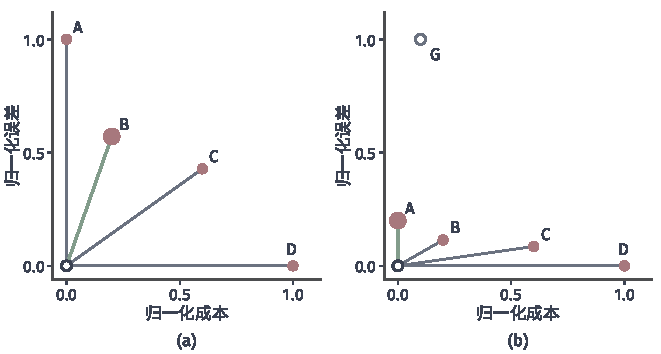
\includegraphics[width=112mm]{figures/05-optimization/07-multiple-criteria-and-nested-optimization/matplotlib/moo-scale-range/figure.pdf}
  \caption{参考范围对归一化比较的影响。线段是各方案到理想点（原点）的距离，绿色线段是最短的一条，大圆点是被选中的方案。(a)以$A,B,C,D$的范围归一化，选$B$。(b)候选中混入被支配的$G=(1.5,36)$，误差范围变大，选$A$。}
  \label{fig:moo-scale-range}
\end{BookInlineFigure}

这里的教训有两条。凡是用到权重或距离的比较，都要写明所用的单位或参考范围。归一化不是中性的操作，它把“一单位误差值多少钱”换成了“各目标范围的一格彼此相当”，这也是一种偏好，只是不那么显眼。参考范围最好由被信任的方案决定，并在结果中报告，不让被支配的候选参与定尺度。

\section{标量化}
\label{sec:moo-scalarization}

决策者往往能说出某种偏好：一项指标值多少钱，或者预算不能超过多少，或者希望各项都接近某个水平。有了偏好，就可以把多目标问题改写成单目标问题，再调用前面各章的方法。这样的改写称为\term{标量化}（scalarization）。

每种改写的解是不是Pareto最优点？改写的参数变化时，能到达前沿上的哪些点？要记住的一点是，标量化问题的解只代表这一次写下的偏好，不是“多目标问题的解”。

\subsection{加权和}
\label{sec:moo-weighted}

最直接的偏好是价格：给每个目标定一个单价，只看总价。这一小节研究按总价选出的方案有什么性质，以及扫遍所有价格能不能走遍前沿。

\paragraph{定义与直观}
取权重$\bm{w}$属于单纯形
\[
 \Delta_m=\Bigl\{\bm{w}\in\mathbb{R}^m:w_i\geq0,\ \sum_{i=1}^mw_i=1\Bigr\},
\]
求解
\begin{equation}
 \min_{\bm{x}\in\bm{C}}\ \sum_{i=1}^mw_if_i(\bm{x}).
 \label{eq:moo-weighted}
\end{equation}
这种做法称为\term{加权和法}（weighted-sum method）。两个目标时，把权重简写成$\bm{w}=(w,1-w)$，$w\in[0,1]$。

在目标平面上，总价相同的点组成一条法向为$\bm{w}$的直线。最小化总价，就是让这条直线从左下方平移过来，直到第一次碰到可达目标集。碰到的点就是解，这条直线称为\term{支撑线}（supporting line）。下面的讨论几乎都从这幅图景得来，见图~\ref{fig:moo-weighted-support}。

\begin{BookInlineFigure}
  \centering
  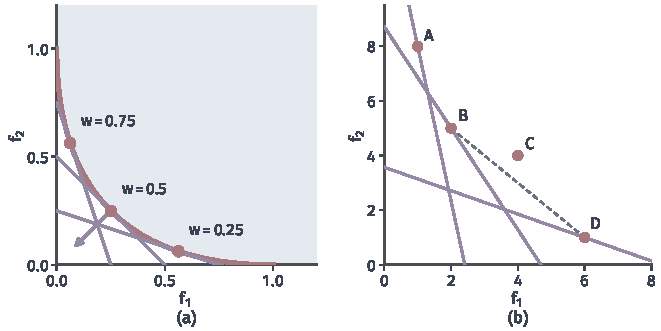
\includegraphics[width=112mm]{figures/05-optimization/07-multiple-criteria-and-nested-optimization/matplotlib/moo-weighted-support/figure.pdf}
  \caption{加权和的支撑线，紫线是最低的等总价线。(a)式~\eqref{eq:moo-iso}的前沿（红色），$w=0.25,0.5,0.75$时的切点；紫色箭头是$w=0.5$时的负法向，指向总价下降的方向。(b)式~\eqref{eq:moo-candidates}中$A,B,C,D$四点，$w=0.3,0.65,0.85$的支撑线分别经过$D,B,A$；$C$在虚线$BD$上方，任何支撑线都先碰到别的点。}
  \label{fig:moo-weighted-support}
\end{BookInlineFigure}

\paragraph{加权和的解与Pareto最优}
解的性质由权重的符号决定。权重全正时，支配者在总价上一定严格更便宜，所以解不会被支配。权重有零时，零权重目标的严格改善不计入总价，只能得到较弱的结论。

\begin{theorem}[加权和的解]
\label{thm:moo-weighted}
设$\bm{x}^\star$是问题~\eqref{eq:moo-weighted}的全局最优解。
\begin{enumerate}
 \item 若所有$w_i>0$，则$\bm{x}^\star$是Pareto最优点。
 \item 若$\bm{w}\in\Delta_m$，则$\bm{x}^\star$是弱Pareto最优点。
 \item 若$\bm{w}\in\Delta_m$，且$\bm{x}^\star$是问题~\eqref{eq:moo-weighted}的唯一全局最优解，则$\bm{x}^\star$是Pareto最优点。
\end{enumerate}
\end{theorem}

\begin{proof}
记$\phi(\bm{x})=\sum_iw_if_i(\bm{x})$。

(1)若$\bm{u}\in\bm{C}$支配$\bm{x}^\star$，则$w_if_i(\bm{u})\leq w_if_i(\bm{x}^\star)$对所有$i$成立。对$f_i(\bm{u})<f_i(\bm{x}^\star)$的那个$i$，由$w_i>0$得严格不等号。逐项相加得$\phi(\bm{u})<\phi(\bm{x}^\star)$，矛盾。

(2)若$\bm{u}\in\bm{C}$使$f_i(\bm{u})<f_i(\bm{x}^\star)$对所有$i$成立，由于$\bm{w}\in\Delta_m$，至少有一个$w_i>0$，相加仍得$\phi(\bm{u})<\phi(\bm{x}^\star)$，矛盾。

(3)若$\bm{u}\in\bm{C}$支配$\bm{x}^\star$，由$w_i\geq0$得$\phi(\bm{u})\leq\phi(\bm{x}^\star)$，所以$\bm{u}$也是全局最优解。由唯一性$\bm{u}=\bm{x}^\star$，这与“至少一项严格更小”矛盾。
\end{proof}

三条结论都只用到全局最优性，没有用到凸性。定理的第~1条马上回答了第~\ref{sec:moo-pareto}节留下的存在性问题。

\begin{theorem}[Pareto最优点的存在]
\label{thm:moo-existence}
设$\bm{C}$非空紧，各$f_i$在$\bm{C}$上连续，则Pareto解集非空。
\end{theorem}

\begin{proof}
取$w_i=1/m$。连续函数$\sum_iw_if_i$在非空紧集上取得最小值，这是第~\ref{chap:optimization}章的结论。由定理~\ref{thm:moo-weighted}的第~1条，最小点是Pareto最优点。
\end{proof}

第~\ref{sec:moo-pareto}节的反例中$\bm{C}=(0,1]$不闭，紧性不成立。

\paragraph{连续例：权重到前沿的对应}
对例~\eqref{eq:moo-iso}，由式~\eqref{eq:moo-iso-coords}，总价是
\[
 w\,s^2+(1-w)(1-s)^2+\tfrac12r^2.
\]
先取$r=0$，再对$s$求导令其为零：
\[
 2ws-2(1-w)(1-s)=0.
\]
解得$s=1-w$，也就是$\bm{x}=(w,1-w)$，对应前沿上的点
\begin{equation}
 \bigl(f_1,f_2\bigr)=\bigl((1-w)^2,\ w^2\bigr).
 \label{eq:moo-iso-weighted}
\end{equation}

前沿在该点的斜率也能算出来。由式~\eqref{eq:moo-iso-front}，$\mathrm{d}f_2/\mathrm{d}f_1=-(1-s)/s=-w/(1-w)$，正好等于等总价线的斜率。价格比决定了切点的位置，这就是图~\ref{fig:moo-weighted-support}(a)显示的情况。

例如$w=1/2$时，解是$\bm{x}=(1/2,1/2)$，目标是$(1/4,1/4)$。端点$\bm{x}=\bm{a}$只有在$w=1$时才能得到，此时权重有零，但解唯一，由定理~\ref{thm:moo-weighted}的第~3条它仍是Pareto最优点。

\paragraph{有限例：下包络}
对式~\eqref{eq:moo-candidates}，每个候选的总价是$w$的一次函数：
\[
 \begin{gathered}
  A:\ 8-7w,\quad B:\ 5-3w,\quad C:\ 4,\\
  D:\ 1+5w,\quad E:\ 6-w,\quad F:\ 1+6w.
 \end{gathered}
\]
图~\ref{fig:moo-weighted-envelope}把六条直线画在一起，每个$w$上的最小值组成红色的下包络。$w<1/2$时$D$最便宜，$1/2<w<3/4$时$B$最便宜，$w>3/4$时$A$最便宜。

\begin{BookInlineFigure}
  \centering
  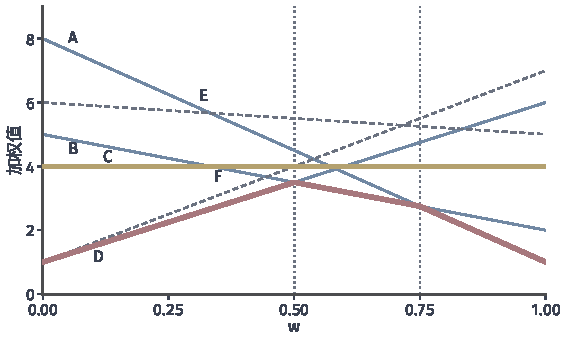
\includegraphics[width=96mm]{figures/05-optimization/07-multiple-criteria-and-nested-optimization/matplotlib/moo-weighted-envelope/figure.pdf}
  \caption{六个候选的总价随权重$w$的变化。红线是下包络，其转折点在$w=1/2$和$w=3/4$。黄线是$C$，它始终在下包络之上。虚线是被支配的$E$和$F$。}
  \label{fig:moo-weighted-envelope}
\end{BookInlineFigure}

$C$虽然是Pareto最优点，却永远选不上。要比$B$便宜，需要$4\leq5-3w$，即$w\leq1/3$；要比$D$便宜，需要$4\leq1+5w$，即$w\geq3/5$。两个要求不能同时满足。

几何上，线段$BD$在$f_1=4$处的高度是$3$，而$C$的高度是$4$，$C$位于线段上方。能被某组权重选中的Pareto点称为\term{支撑点}（supported point），$C$不是支撑点。

下包络也说明了解的跳变：$w$从小到大扫过$1/2$时，答案从$D$直接跳到$B$，两者的总价都是$3.5$；扫过$3/4$时从$B$跳到$A$，总价都是$2.75$。

零权重的情形也可以在这里看到。$w=0$时总价就是误差，$D$和$F$都等于$1$，并列最优，而$F$被$D$支配。定理~\ref{thm:moo-weighted}只保证$F$是弱Pareto最优点，这个结论不能再加强。

\paragraph{凸问题：非负权重足够覆盖}
前面的例子表明，非凸时支撑点可能不是全部。凸性保证的是，不存在$C$那样藏在凹陷里的点。

\begin{theorem}[凸问题的支撑权重]
\label{thm:moo-convex-support}
设$\bm{C}$凸，各$f_i$在$\bm{C}$上凸。若$\bar{\bm{x}}$是全局弱Pareto最优点，则存在$\bm{w}\in\Delta_m$，使$\bar{\bm{x}}$是问题~\eqref{eq:moo-weighted}的全局最优解。
\end{theorem}

证明的思路是把可达集合向右上方“加厚”，使它成为凸集，再用超平面把它与$\bar{\bm{y}}$左下方的点隔开。所用的严格分离定理在第~\ref{chap:duality}章已经证明：一点若不在闭凸集中，就存在超平面把二者严格分开。

\begin{proof}
记$\bar{\bm{y}}=\bm{f}(\bar{\bm{x}})$，记全$1$向量为$\bm{1}$。令
\[
 \bm{A}=\{\bm{f}(\bm{x})+\bm{t}:\bm{x}\in\bm{C},\ \bm{t}\geq\bm{0}\}.
\]

先说明$\bm{A}$凸。取$\bm{f}(\bm{x})+\bm{t}$与$\bm{f}(\bm{x}')+\bm{t}'$，$\gamma\in[0,1]$。由$f_i$凸，
\[
 \bm{f}(\gamma\bm{x}+(1-\gamma)\bm{x}')\leq\gamma\bm{f}(\bm{x})+(1-\gamma)\bm{f}(\bm{x}'),
\]
差额并入$\bm{t}$的凸组合，所以这两点的凸组合仍在$\bm{A}$中。于是闭包$\operatorname{cl}\bm{A}$是闭凸集。

对$\epsilon>0$，点$\bm{z}_\epsilon=\bar{\bm{y}}-\epsilon\bm{1}$不在$\operatorname{cl}\bm{A}$中。否则有$\bm{A}$中的点列趋于$\bm{z}_\epsilon$，其中某一点的每个分量都严格小于$\bar{\bm{y}}$的相应分量。这个点形如$\bm{f}(\bm{x})+\bm{t}$，于是$f_i(\bm{x})<\bar{y}_i$对所有$i$成立，与弱Pareto最优矛盾。

由严格分离定理，取单位向量$\bm{c}_\epsilon$，使对所有$\bm{x}\in\bm{C}$，$\bm{t}\geq\bm{0}$，
\[
 \langle\bm{c}_\epsilon,\bm{f}(\bm{x})+\bm{t}\rangle>\langle\bm{c}_\epsilon,\bm{z}_\epsilon\rangle.
\]
若$\bm{c}_\epsilon$有负分量，让$\bm{t}$的相应分量趋于无穷，左端趋于$-\infty$，矛盾，所以$\bm{c}_\epsilon\geq\bm{0}$。

单位球面紧，取$\epsilon\downarrow0$的子列使$\bm{c}_\epsilon\to\bm{c}$。则$\bm{c}\geq\bm{0}$，$\bm{c}\neq\bm{0}$。在上式中取$\bm{t}=\bm{0}$，令$\epsilon\downarrow0$，得到
\[
 \langle\bm{c},\bm{f}(\bm{x})\rangle\geq\langle\bm{c},\bar{\bm{y}}\rangle\quad\text{对所有}\ \bm{x}\in\bm{C}.
\]
令$\bm{w}=\bm{c}/\sum_ic_i\in\Delta_m$，上式就是$\bar{\bm{x}}$最小化$\sum_iw_if_i$。
\end{proof}

定理的结论是“存在非负权重”，不是“存在全正权重”。例~\eqref{eq:moo-iso}的端点$\bm{a}$只有权重$(1,0)$能选中，就说明全正的要求一般做不到。定理的条件也不能去掉，图~\ref{fig:moo-weighted-nonconvex}的两个例子都不满足凸性。

\paragraph{非凸前沿上的遗漏}
第三个例子是一个一元问题：$x\in[0,1]$，
\begin{equation}
 f_1(x)=x,\qquad f_2(x)=1-x^2.
 \label{eq:moo-concave}
\end{equation}
$f_1$递增，$f_2$递减，所以每个$x$都是Pareto最优点，前沿是向右上方鼓起的抛物线。加权目标是
\[
 w\,x+(1-w)(1-x^2).
\]
它是$x$的凹函数，在区间上的最小值只能在端点取到，分别是$x=0$时的$1-w$和$x=1$时的$w$。

于是$w>1/2$时解是$x=0$，$w<1/2$时解是$x=1$，$w=1/2$时两端并列。无论权重取什么，中间的方案都选不到。图~\ref{fig:moo-weighted-nonconvex}(a)中三条紫线都只能碰到两个端点。

\begin{BookInlineFigure}
  \centering
  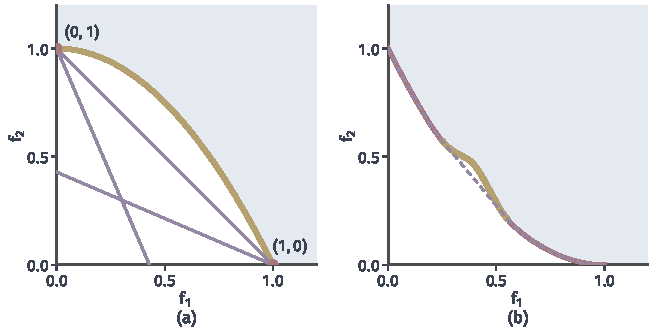
\includegraphics[width=112mm]{figures/05-optimization/07-multiple-criteria-and-nested-optimization/matplotlib/moo-weighted-nonconvex/figure.pdf}
  \caption{加权和遗漏的前沿。(a)式~\eqref{eq:moo-concave}的前沿，紫线是$w=0.3,0.5,0.7$的支撑线，都只碰到端点（红点），黄色段上的点都选不到。(b)带凹陷的前沿$f_2=(1-f_1)^2+0.1\exp(-((f_1-0.4)/0.1)^2)$，紫色虚线是它的下凸包，黄色段（$0.25<f_1<0.55$）位于凸包上方，选不到。}
  \label{fig:moo-weighted-nonconvex}
\end{BookInlineFigure}

现实中的前沿常常只有一段凹陷。图~\ref{fig:moo-weighted-nonconvex}(b)中，前沿由一个下凸的主体和一个小鼓包组成。任何方向的支撑线都不会碰到黄色段内部，紫色虚线就是它的\term{下凸包}（lower convex hull），凹陷中的点都比这条线高。从图上也可以知道，权重一旦扫过黄色段两端所对应的斜率，答案就从一端跳到另一端。

所以，“扫描权重”只能得到支撑点。对非凸问题，这可能漏掉前沿的大部分。

\subsection{阈值约束}
\label{sec:moo-threshold}

很多需求本来就不是价格，而是硬指标：预算不超过某个数，在此前提下误差尽量小。这一小节把这种需求写成约束，研究它和加权和有什么不同。

\paragraph{定义}
保留第$j$个目标作为被最小化的量，其余目标用阈值$\tau_i$限制：
\begin{equation}
 \min_{\bm{x}\in\bm{C}}\ f_j(\bm{x})
 \quad\text{s.t.}\quad f_i(\bm{x})\leq\tau_i,\ \ i\neq j.
 \label{eq:moo-threshold}
\end{equation}
这种做法称为\term{阈值约束法}（$\varepsilon$-constraint method）。这是一个普通的约束优化问题，第~\ref{chap:constrained-optimality}章的最优性条件和前一部分各章的求解方法都能直接用上。

在目标平面上，两个目标时阈值约束是一条竖线$f_1\leq\tau$，竖线左侧的部分是可行的，问题就是在其中找最低点。这条竖线不需要从外部支撑可达集合，所以能插进前沿的凹陷里。

\paragraph{解的性质}
和加权和不同，这里的结论有反方向的一半，而且不需要凸性。

\begin{theorem}[阈值约束的解]
\label{thm:moo-threshold}
固定$j$与阈值$\tau_i$，$i\neq j$。
\begin{enumerate}
 \item 问题~\eqref{eq:moo-threshold}的每个全局最优解都是弱Pareto最优点；若全局最优解唯一，它是Pareto最优点。
 \item 若$\bar{\bm{x}}$是Pareto最优点，取$\tau_i=f_i(\bar{\bm{x}})$，$i\neq j$，则$\bar{\bm{x}}$是问题~\eqref{eq:moo-threshold}的全局最优解。
 \item 设$\bm{S}$是问题~\eqref{eq:moo-threshold}的全局最优解集。若$\tilde{\bm{x}}$在$\bm{S}$上最小化$\sum_{i\neq j}f_i$，则$\tilde{\bm{x}}$是Pareto最优点。
\end{enumerate}
\end{theorem}

\begin{proof}
(1)设$\hat{\bm{x}}$是全局最优解。若$\bm{u}\in\bm{C}$的各目标都严格小于$\hat{\bm{x}}$，则$f_i(\bm{u})<f_i(\hat{\bm{x}})\leq\tau_i$，$\bm{u}$可行，而$f_j(\bm{u})<f_j(\hat{\bm{x}})$，矛盾。

若$\hat{\bm{x}}$是唯一全局最优解，设$\bm{u}$支配$\hat{\bm{x}}$。同样$\bm{u}$可行，且$f_j(\bm{u})\leq f_j(\hat{\bm{x}})$，所以$\bm{u}$也是全局最优解。由唯一性$\bm{u}=\hat{\bm{x}}$，与支配矛盾。

(2)$\bar{\bm{x}}$满足$f_i(\bar{\bm{x}})\leq\tau_i$，可行。若可行点$\bm{u}$使$f_j(\bm{u})<f_j(\bar{\bm{x}})$，再由可行性$f_i(\bm{u})\leq\tau_i=f_i(\bar{\bm{x}})$，$\bm{u}$支配$\bar{\bm{x}}$，矛盾。

(3)设$\bm{u}\in\bm{C}$支配$\tilde{\bm{x}}$。各约束下$f_i(\bm{u})\leq f_i(\tilde{\bm{x}})\leq\tau_i$，$\bm{u}$可行；又$f_j(\bm{u})\leq f_j(\tilde{\bm{x}})$，所以$\bm{u}\in\bm{S}$，且$f_j(\bm{u})=f_j(\tilde{\bm{x}})$。于是严格减小的分量在$i\neq j$中，$\sum_{i\neq j}f_i(\bm{u})<\sum_{i\neq j}f_i(\tilde{\bm{x}})$，矛盾。
\end{proof}

第~2条说的是，每个Pareto点都能被某组阈值选中，即使它不是支撑点。第~3条给出处理并列最优解的办法：先满足阈值并最小化$f_j$，再在并列的解中比较其余目标。这种分步择优也叫字典序的处理。

\paragraph{有限例与不可行}
在式~\eqref{eq:moo-candidates}上取$j=2$，以成本为预算$\tau$，求误差的最小值
\begin{equation}
 v(\tau)=\min\{f_2:f_1\leq\tau\}.
 \label{eq:moo-threshold-value}
\end{equation}
逐段比较得到：
\[
 v(\tau)=
 \begin{cases}
  \text{不可行},&\tau<1,\\
  8\ (A),&1\leq\tau<2,\\
  5\ (B),&2\leq\tau<4,\\
  4\ (C),&4\leq\tau<6,\\
  1\ (D),&\tau\geq6.
 \end{cases}
\]

这张表说明了三件事。阈值过紧时问题不可行，应当如实报告“不存在满足要求的方案”，不要输出一个违反约束的点。预算扫过$4$时选中了$C$，这个点加权和永远选不到。$\tau\geq7$时$D$与$F$并列，而$F$被$D$支配，这时按定理~\ref{thm:moo-threshold}的第~3条再比较成本，就排除了$F$。

\begin{BookInlineFigure}
  \centering
  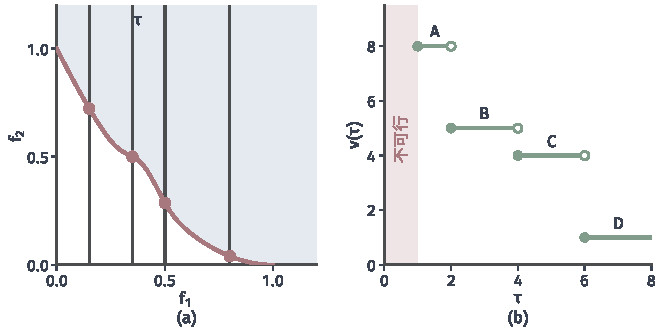
\includegraphics[width=112mm]{figures/05-optimization/07-multiple-criteria-and-nested-optimization/matplotlib/moo-threshold-scan/figure.pdf}
  \caption{阈值约束的扫描。(a)图~\ref{fig:moo-weighted-nonconvex}(b)的前沿，深灰竖线是四个阈值，红点是相应的解，其中两个点在加权和选不到的凹陷段内。(b)有限例的$v(\tau)$，实心点属于该段，空心点不属于；粉色区域不可行，字母是选中的方案。}
  \label{fig:moo-threshold-scan}
\end{BookInlineFigure}

图~\ref{fig:moo-threshold-scan}(a)显示，阈值从左向右扫过时，解沿整条前沿移动。代价是每次都要解一个带约束的问题，这比加权和难：加权和只是一个无约束问题，这里多了一个可能起作用的约束。

\paragraph{阈值与价格的联系}
阈值$\tau$和价格$w$看起来是两种语言，通过乘子可以把它们联系起来。把例~\eqref{eq:moo-iso}写成$j=2$的阈值问题，
\[
 \min\ f_2(\bm{x})\quad\text{s.t.}\quad f_1(\bm{x})\leq\tau,
\]
约束起作用时，KKT驻定条件（第~\ref{chap:constrained-optimality}章）要求
\begin{equation}
 \nabla f_2(\bm{x})+\lambda\nabla f_1(\bm{x})=\bm{0},\qquad\lambda\geq0.
 \label{eq:moo-threshold-kkt}
\end{equation}

式~\eqref{eq:moo-threshold-kkt}除以$1+\lambda$，就是权重$\bm{w}=(\lambda,1)/(1+\lambda)$的加权和的驻定条件。乘子$\lambda$就是目标$f_1$相对于$f_2$的价格。

具体计算。在解的线段上$f_1=s^2=\tau$，所以$s=\sqrt\tau$，且$r=0$。式~\eqref{eq:moo-threshold-kkt}沿线段方向的分量给出$(s-1)+\lambda s=0$，于是
\begin{equation}
 \lambda(\tau)=\frac{1-\sqrt\tau}{\sqrt\tau},\qquad 0<\tau\leq1.
 \label{eq:moo-iso-lambda}
\end{equation}

例如$\tau=1/4$时，$s=1/2$，$\lambda=1$，权重正是$(1/2,1/2)$，解与式~\eqref{eq:moo-iso-weighted}中$w=1/2$的解相同。

式~\eqref{eq:moo-iso-lambda}也描述了$\tau$增大时价格怎样变化。由式~\eqref{eq:moo-iso-front}，最优值$v(\tau)=(1-\sqrt\tau)^2$，求导得
\[
 v'(\tau)=-\frac{1-\sqrt\tau}{\sqrt\tau}=-\lambda(\tau).
\]
放宽一单位阈值，最优值下降$\lambda$，这与第~\ref{chap:parametric-sensitivity}章乘子是影子价格的结论一致。图~\ref{fig:moo-threshold-price}画出了这一点。$\tau$接近$0$时$\lambda$趋于无穷，$\tau\geq1$时约束不再起作用，$\lambda=0$，解停在$\bm{b}$。

\begin{BookInlineFigure}
  \centering
  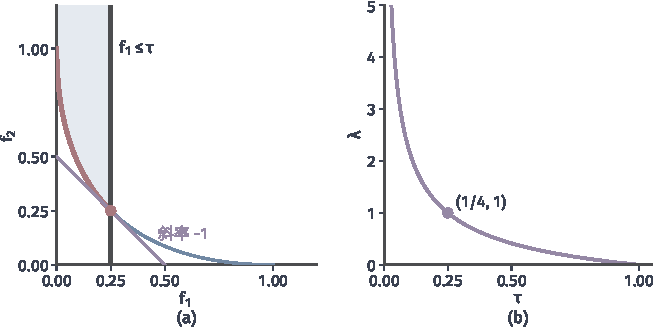
\includegraphics[width=112mm]{figures/05-optimization/07-multiple-criteria-and-nested-optimization/matplotlib/moo-threshold-price/figure.pdf}
  \caption{阈值与价格，例~\eqref{eq:moo-iso}。(a)深灰竖线是阈值$f_1\leq1/4$，可行部分为左侧浅蓝区域，红色段是可行的前沿，红点是解；紫线是前沿在该点的切线，斜率$-\lambda=-1$。(b)乘子随阈值的变化，式~\eqref{eq:moo-iso-lambda}。}
  \label{fig:moo-threshold-price}
\end{BookInlineFigure}

这种对应只在问题有相应结构时才是一一对应。非凸时，凹陷中的解仍满足式~\eqref{eq:moo-threshold-kkt}，但它只是相应加权和的驻定点，不是最小点。阈值问题的解能到达加权和到不了的地方，正是因为这里的约束替代了全局的比较。

\paragraph{并列最优解}
前沿出现水平段时，阈值问题的解不唯一。图~\ref{fig:moo-threshold-tie}中，阈值$\tau$落在底部水平边的范围内，$\bm{z}'$和$\bm{z}$的$f_2$都等于最小值，黄色线段上的点都是最优解。$\bm{z}$被$\bm{z}'$支配。

\begin{BookInlineFigure}
  \centering
  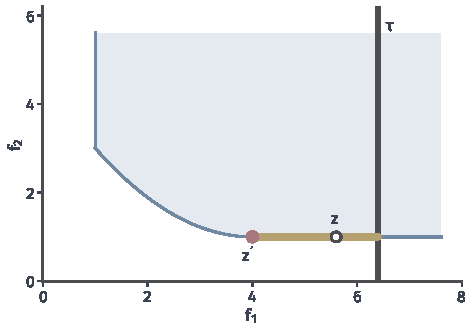
\includegraphics[width=80mm]{figures/05-optimization/07-multiple-criteria-and-nested-optimization/matplotlib/moo-threshold-tie/figure.pdf}
  \caption{阈值约束的并列最优解。深灰竖线是阈值，黄色线段是$\min\{f_2:f_1\leq\tau\}$的全部解的目标值。空心点$\bm{z}$是弱Pareto最优点，红点$\bm{z}'$是在并列解中进一步最小化$f_1$后得到的Pareto最优点。}
  \label{fig:moo-threshold-tie}
\end{BookInlineFigure}

求解器一般只返回并列解中的某一个，不一定是$\bm{z}'$。所以，只要阈值问题的解不能确认唯一，就要做第二阶段的择优，否则报告的只是一个弱Pareto最优点。

\subsection{参考点方法}
\label{sec:moo-reference}

有时决策者说的既不是价格，也不是预算，而是希望各项指标都接近某个水平。这一小节把这种需求写成到参考点的最大偏差，它能选中加权和选不到的点，又不必增加约束。

\paragraph{定义}
设各目标在$\bm{C}$上有有限下界，取\term{参考点}（reference point）$\bm{z}$，使$z_i<\inf_{\bm{C}}f_i$对所有$i$成立。再取权重$w_i>0$，最小化带权的最大偏差：
\begin{equation}
 \min_{\bm{x}\in\bm{C}}\ \max_{1\leq i\leq m}\ w_i\bigl(f_i(\bm{x})-z_i\bigr).
 \label{eq:moo-chebyshev}
\end{equation}
这种做法称为\term{加权Chebyshev标量化}（weighted Chebyshev scalarization）。

式~\eqref{eq:moo-chebyshev}的直观含义是，目标被缩放后，看离参考点最远的一项。下水平集是以$\bm{z}$为左下角的长方形，边长比由权重决定。随着水平增大，长方形的右上角沿着从$\bm{z}$出发、方向为$(1/w_1,\ldots,1/w_m)$的射线向外移动。长方形第一次碰到可达集合时的水平，就是最优值。

长方形的右上角尖尖地探出去，而加权和的直线是平的。平的直线碰不到凹陷，尖的角能探进去，见图~\ref{fig:moo-chebyshev-level}。

\begin{BookInlineFigure}
  \centering
  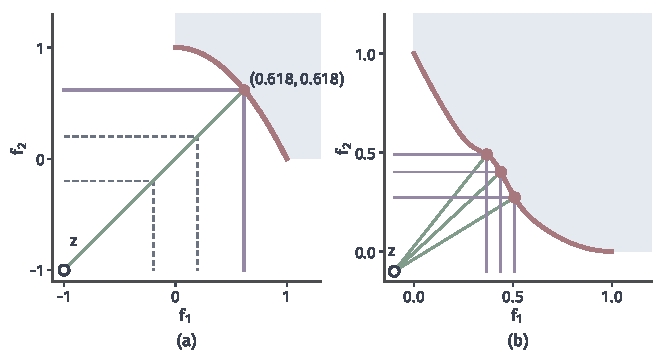
\includegraphics[width=112mm]{figures/05-optimization/07-multiple-criteria-and-nested-optimization/matplotlib/moo-chebyshev-level/figure.pdf}
  \caption{加权Chebyshev的水平集，空心点是参考点$\bm{z}$，绿线是沿$(1/w_1,1/w_2)$的射线。(a)式~\eqref{eq:moo-concave}的前沿，$\bm{z}=(-1,-1)$，$\bm{w}=(1/2,1/2)$；灰色虚线是较低水平的长方形边界，紫线是最优水平，角落碰到$(0.618,0.618)$。(b)图~\ref{fig:moo-weighted-nonconvex}(b)的前沿，$\bm{z}=(-0.1,-0.1)$，三组权重的解都在凹陷段内，紫线是相应的最优长方形边界。}
  \label{fig:moo-chebyshev-level}
\end{BookInlineFigure}

\paragraph{解的性质}
先看式~\eqref{eq:moo-chebyshev}的解是什么点，再看能选到哪些点。

\begin{theorem}[加权Chebyshev的解]
\label{thm:moo-chebyshev}
设$\bm{z}$严格低于各目标的下确界。
\begin{enumerate}
 \item 对任意$w_i>0$，问题~\eqref{eq:moo-chebyshev}的全局最优解都是弱Pareto最优点。
 \item 若$\bar{\bm{x}}$是弱Pareto最优点，取
 \begin{equation}
  w_i=\frac{1}{f_i(\bar{\bm{x}})-z_i},
  \label{eq:moo-chebyshev-weight}
 \end{equation}
 则$\bar{\bm{x}}$是问题~\eqref{eq:moo-chebyshev}的全局最优解。
 \item 设$\bm{S}$是问题~\eqref{eq:moo-chebyshev}的全局最优解集。若$\tilde{\bm{x}}$在$\bm{S}$上最小化$\sum_if_i$，则$\tilde{\bm{x}}$是Pareto最优点。
\end{enumerate}
\end{theorem}

\begin{proof}
记$\psi(\bm{x})=\max_iw_i(f_i(\bm{x})-z_i)$。

(1)设$\bm{x}^\star$是全局最优解。若$\bm{u}$的各目标都严格小于$\bm{x}^\star$，由$w_i>0$，对所有$i$有
\[
 w_i(f_i(\bm{u})-z_i)<w_i(f_i(\bm{x}^\star)-z_i)\leq\psi(\bm{x}^\star).
\]
有限个严格不等式取最大仍严格，$\psi(\bm{u})<\psi(\bm{x}^\star)$，矛盾。

(2)由$z_i<\inf f_i$，式~\eqref{eq:moo-chebyshev-weight}中分母为正，$w_i>0$，并且
\[
 w_i\bigl(f_i(\bar{\bm{x}})-z_i\bigr)=1\quad\text{对所有}\ i,
\]
所以$\psi(\bar{\bm{x}})=1$。若有$\bm{u}$使$\psi(\bm{u})<1$，则$w_i(f_i(\bm{u})-z_i)<1$对所有$i$成立，代入$w_i$的定义得$f_i(\bm{u})<f_i(\bar{\bm{x}})$对所有$i$成立，与弱Pareto最优矛盾。

(3)设$\bm{u}$支配$\tilde{\bm{x}}$。各项$f_i(\bm{u})\leq f_i(\tilde{\bm{x}})$，由$w_i>0$得$\psi(\bm{u})\leq\psi(\tilde{\bm{x}})$，所以$\bm{u}\in\bm{S}$。又有一项严格减小，$\sum_if_i(\bm{u})<\sum_if_i(\tilde{\bm{x}})$，矛盾。
\end{proof}

$\bm{z}$严格低于下确界的条件保证了第~2条的权重有限且为正。第~2条不需要凸性，这也是这种标量化比加权和强的地方：调整权重可以选中每一个弱Pareto最优点，当然也包括每一个Pareto最优点。

\paragraph{算一个连续的例子}
对式~\eqref{eq:moo-concave}取$\bm{z}=(-1,-1)$，它低于两个目标的下确界$0$。取$\bm{w}=(1/2,1/2)$，目标是
\[
 \psi(x)=\frac12\max\bigl\{x+1,\ 2-x^2\bigr\}.
\]
$x+1$递增，$2-x^2$递减，最大值的最小点在两者相等处：
\[
 x+1=2-x^2,\quad\text{即}\quad x^2+x-1=0.
\]
解得$x=(\sqrt5-1)/2\approx0.618$，目标向量也是$(0.618,0.618)$，这是加权和选不到的中间点。

\paragraph{有限例：并列最优仍会发生}
在式~\eqref{eq:moo-candidates}上取$\bm{z}=(0,0)$，它严格低于下确界$(1,1)$。取$\bm{w}=(1/2,1/2)$，各候选的$\psi$值为
\[
 A:\ 4,\quad B:\ 2.5,\quad C:\ 2,\quad D:\ 3,\quad E:\ 3,\quad F:\ 3.5.
\]
最小的是$C$，这正是加权和选不到的方案，见图~\ref{fig:moo-chebyshev-finite}(a)。

再取$\bm{w}=(0.1,0.9)$，各候选的$\psi$值为
\[
 A:\ 7.2,\quad B:\ 4.5,\quad C:\ 3.6,\quad D:\ 0.9,\quad E:\ 5.4,\quad F:\ 0.9.
\]
$D$与$F$并列最小。此时第二个目标的偏差决定了最大值，第一个目标的差别被$\max$吞掉了，$F$虽然被$D$支配，却同样最优，见图~\ref{fig:moo-chebyshev-finite}(b)。按定理~\ref{thm:moo-chebyshev}的第~3条再比较$\sum_if_i$，$D$的和是$7$，$F$的和是$8$，排除了$F$。

\begin{BookInlineFigure}
  \centering
  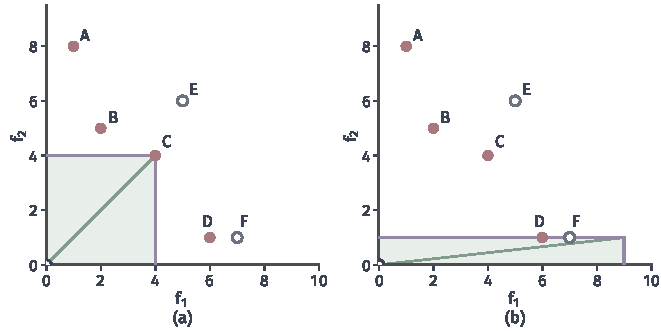
\includegraphics[width=112mm]{figures/05-optimization/07-multiple-criteria-and-nested-optimization/matplotlib/moo-chebyshev-finite/figure.pdf}
  \caption{有限候选上的加权Chebyshev，参考点$\bm{z}=(0,0)$（空心点在原点）。绿色长方形是最优水平的下水平集，紫线是其右上边界。(a)$\bm{w}=(1/2,1/2)$，长方形的角落碰到$C$。(b)$\bm{w}=(0.1,0.9)$，长方形的上边同时碰到$D$和$F$，$F$是并列的弱Pareto最优点。}
  \label{fig:moo-chebyshev-finite}
\end{BookInlineFigure}

\paragraph{三种写法的比较}
表~\ref{tab:moo-scalarization}汇总了三种标量化。没有哪一种处处占优。加权和最容易求解，但只能到达支撑点；阈值约束和加权Chebyshev能到达每个Pareto点，代价是多了约束或非光滑的$\max$。后者可以用第~\ref{chap:quadratic-conic-programming}章一类的上图改写来处理：引入变量$t$，在约束$w_i(f_i(\bm{x})-z_i)\leq t$下最小化$t$。

\begin{BookInlineTable}
  \centering
  \caption{三种标量化的比较。“解的保证”指全局最优解的性质。}
  \label{tab:moo-scalarization}
  \begin{tabular}{@{}llll@{}}
    \toprule
    方法 & 解的保证 & 可达的点 & 并列情形\\
    \midrule
    加权和 & 全正权：Pareto & 支撑点 & 权重有零时\\
    阈值约束 & 弱Pareto & 全部Pareto点 & 水平段上\\
    加权Chebyshev & 弱Pareto & 全部弱Pareto点 & 水平段或竖直段\\
    \bottomrule
  \end{tabular}
\end{BookInlineTable}

这些结论的更多变形可以查阅凸优化专著中多准则优化一节\scite{math-boyd2004convex}。无论用哪一种，所得的都只是一次偏好下的解。要给决策者看一组候选，还需要第~\ref{sec:moo-front-computation}节的组织方式。

\section{最优解的判别}
\label{sec:moo-optimality}

标量化回答的是“给定偏好求一个解”。这一节换一个问法：手里已经有一个候选点，只看它附近的导数信息，能否判断它值不值得继续改进？

单目标问题中，这个问题由“存在下降方向”来回答。多目标问题中对应的问题是：是否存在一个可行的小步，使所有目标都下降？本节先在无约束内点回答，再加上约束。全节都要把两种结论分开：不存在共同下降方向是一个局部的必要条件，它要成为全局Pareto最优的证据，还需要凸性和权重条件。

\subsection{共同下降方向}
\label{sec:moo-common-descent}

设$\bm{x}$是$\bm{C}$的内点，各$f_i$在$\bm{x}$处可微，记
\[
 \bm{g}_i=\nabla f_i(\bm{x}),\qquad i=1,\ldots,m.
\]
我们想知道，从$\bm{x}$出发能不能让全部目标一起变小。

\paragraph{方向的定义}
一个方向$\bm{d}$若满足
\begin{equation}
 \langle\bm{g}_i,\bm{d}\rangle<0\quad\text{对所有}\ i=1,\ldots,m,
 \label{eq:moo-common-descent}
\end{equation}
就称为\term{共同下降方向}（common descent direction）。由一阶Taylor展开，沿这样的$\bm{d}$走足够小的一步，每个目标都严格下降，当前点就被支配了。

每个不等式要求$\bm{d}$落在以$\bm{g}_i$为法向的一个开半空间内，所有这些半空间的公共部分就是全部共同下降方向。图~\ref{fig:moo-common-descent}(a)中两个梯度夹角小于$180^\circ$，绿色楔形就是这个公共部分。

等高线上的直观是：站在山坡上，每个目标各有一个下山的半平面。几个半平面还有公共的部分，就能一步同时往几座山的下坡方向走。公共部分消失时，不管往哪里走，至少有一个目标的一阶变化不是下降。

\begin{BookInlineFigure}
  \centering
  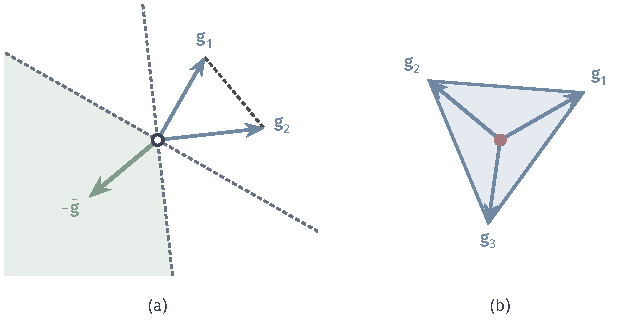
\includegraphics[width=104.8mm]{figures/05-optimization/07-multiple-criteria-and-nested-optimization/tikz/moo-common-descent/figure.pdf}
  \caption{共同下降方向与梯度的凸包，空心点和红点是原点。(a)两个梯度的凸包是虚线线段，不含原点；两条灰色虚线分别垂直于$\bm{g}_1,\bm{g}_2$，绿色楔形是共同下降方向。(b)三个梯度的凸包是浅蓝三角形，原点（红点）在其内部，此时不存在共同下降方向。}
  \label{fig:moo-common-descent}
\end{BookInlineFigure}

\paragraph{用梯度的凸包判别}
图~\ref{fig:moo-common-descent}提示了判别方法。把各梯度当作点，看它们的\term{凸包}（convex hull）
\[
 \operatorname{conv}\{\bm{g}_1,\ldots,\bm{g}_m\}=\Bigl\{\sum_{i=1}^m\theta_i\bm{g}_i:\bm{\theta}\in\Delta_m\Bigr\},
\]
也就是全部梯度的加权平均组成的集合。下面的引理说，这个集合是否包含原点，恰好决定共同下降方向是否存在。

\begin{lemma}[共同下降方向的存在性]
\label{lem:moo-gordan}
存在满足式~\eqref{eq:moo-common-descent}的$\bm{d}$，当且仅当$\bm{0}\notin\operatorname{conv}\{\bm{g}_1,\ldots,\bm{g}_m\}$。
\end{lemma}

\begin{proof}
先设$\bm{0}$在凸包中，即有$\bm{\theta}\in\Delta_m$使$\sum_i\theta_i\bm{g}_i=\bm{0}$。若式~\eqref{eq:moo-common-descent}成立，把它们按$\theta_i\geq0$加权相加，由于至少有一个$\theta_i>0$，得到
\[
 0=\Bigl\langle\sum_i\theta_i\bm{g}_i,\bm{d}\Bigr\rangle=\sum_i\theta_i\langle\bm{g}_i,\bm{d}\rangle<0,
\]
矛盾。

再设$\bm{0}$不在凸包中。凸包是非空紧凸集，记原点在它上面的投影为$\bar{\bm{g}}\neq\bm{0}$。第~\ref{chap:nonsmooth-composite-optimization}章的投影性质给出，对凸包中任一点$\bm{v}$，
\[
 \langle\bm{0}-\bar{\bm{g}},\bm{v}-\bar{\bm{g}}\rangle\leq0.
\]
取$\bm{v}=\bm{g}_i$，整理得
\[
 \langle\bm{g}_i,\bar{\bm{g}}\rangle\geq\lVert\bar{\bm{g}}\rVert_2^2>0.
\]
令$\bm{d}=-\bar{\bm{g}}$，式~\eqref{eq:moo-common-descent}成立。
\end{proof}

第二部分的构造不只是存在性证明，第~\ref{sec:moo-mgda}节就要把它变成算法。原点在凸包中的情形有专门的名称。

\begin{definition}[Pareto驻定]
\label{def:moo-stationary}
若存在$\bm{\theta}\in\Delta_m$，使
\begin{equation}
 \sum_{i=1}^m\theta_i\nabla f_i(\bm{x})=\bm{0},
 \label{eq:moo-stationary}
\end{equation}
称$\bm{x}$为\term{Pareto驻定}（Pareto stationary）点。
\end{definition}

$m=1$时，$\theta_1=1$，式~\eqref{eq:moo-stationary}就是$\nabla f_1=\bm{0}$，回到单目标的驻定点。多目标时，并不要求每个梯度为零，只要求它们能以非负系数相互抵消。

\paragraph{必要性与连续例}
局部最优点不允许共同下降，由此得到一阶必要条件。

\begin{theorem}[Pareto驻定的必要性]
\label{thm:moo-stationary-necessary}
设$\bm{x}$是$\bm{C}$的内点，各$f_i$在$\bm{x}$处可微。若$\bm{x}$是局部弱Pareto最优点，特别地若$\bm{x}$是局部Pareto最优点，则$\bm{x}$是Pareto驻定点。
\end{theorem}

\begin{proof}
若$\bm{x}$不是Pareto驻定点，由引理~\ref{lem:moo-gordan}，存在满足式~\eqref{eq:moo-common-descent}的$\bm{d}$。对充分小的$t>0$，由Taylor展开，
\[
 f_i(\bm{x}+t\bm{d})=f_i(\bm{x})+t\langle\bm{g}_i,\bm{d}\rangle+o(t)<f_i(\bm{x})
\]
对所有$i$成立。$\bm{x}$是内点，$\bm{x}+t\bm{d}$可行，这与局部弱Pareto最优矛盾。
\end{proof}

下面在例~\eqref{eq:moo-iso}上检查，见图~\ref{fig:moo-gradient-points}。此时$\bm{g}_1=\bm{x}-\bm{a}$，$\bm{g}_2=\bm{x}-\bm{b}$。在线段外的点$\bm{p}=(1,1)$处，
\[
 \bm{g}_1=(0,1),\qquad\bm{g}_2=(1,0).
\]
它们的凸组合是$(1-\theta,\theta)$，永远不为零，所以$\bm{p}$不是驻定点。取$\theta=1/2$得最短的组合$(1/2,1/2)$，方向$\bm{d}=(-1/2,-1/2)$使两个目标同时下降。

在线段上的点$\bm{q}=(0.6,0.4)$处，
\[
 \bm{g}_1=(-0.4,0.4),\qquad\bm{g}_2=(0.6,-0.6).
\]
两个梯度方向相反，取$\bm{\theta}=(0.6,0.4)$得到$0.6\bm{g}_1+0.4\bm{g}_2=\bm{0}$，$\bm{q}$是驻定点。这里的$\theta_1=0.6$恰好等于式~\eqref{eq:moo-iso-weighted}中选中$\bm{q}$的权重$w$。

\begin{BookInlineFigure}
  \centering
  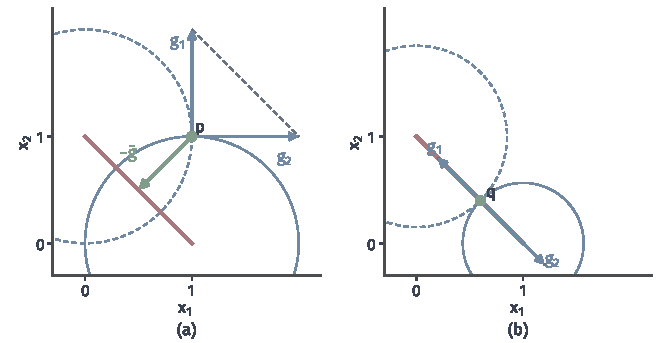
\includegraphics[width=112mm]{figures/05-optimization/07-multiple-criteria-and-nested-optimization/matplotlib/moo-gradient-points/figure.pdf}
  \caption{例~\eqref{eq:moo-iso}中两点处的梯度，圆是经过该点的两条等高线，红色线段是Pareto解集。(a)线段外的点$\bm{p}=(1,1)$，两个梯度的凸包（虚线）不含零，绿色箭头是最小范数组合的反方向。(b)线段上的点$\bm{q}=(0.6,0.4)$，两个梯度反向，凸包含零，两条等高线在$\bm{q}$相切。}
  \label{fig:moo-gradient-points}
\end{BookInlineFigure}

图~\ref{fig:moo-gradient-points}(b)还显示了一件事：在$\bm{q}$处两个圆相切，要进入一个圆的内部，就必须走出另一个圆。这是取舍的局部形象。

\paragraph{驻定点不一定是Pareto最优点}
定理~\ref{thm:moo-stationary-necessary}只有一个方向。Pareto驻定只排除严格的共同下降，并不排除“有的目标不变，另一些目标下降”。取$\bm{x}\in\mathbb{R}^2$，
\begin{equation}
 f_1(\bm{x})=x_1^2,\qquad f_2(\bm{x})=x_2.
 \label{eq:moo-stationary-weak}
\end{equation}
在原点，$\bm{g}_1=\bm{0}$，$\bm{g}_2=(0,1)$，取$\bm{\theta}=(1,0)$，式~\eqref{eq:moo-stationary}成立。可是沿$(0,-t)$移动，$f_1$保持为$0$，$f_2$严格下降，原点被支配，见图~\ref{fig:moo-stationary-gap}(a)。

问题还可能更严重。取一元函数$f_1(x)=f_2(x)=-x^2$，$x=0$是Pareto驻定点，但$x=\pm1$处两个目标都更小，原点连弱Pareto最优点都不是，见图~\ref{fig:moo-stationary-gap}(b)。这与单目标的极大点也是驻定点是同一回事。

\begin{BookInlineFigure}
  \centering
  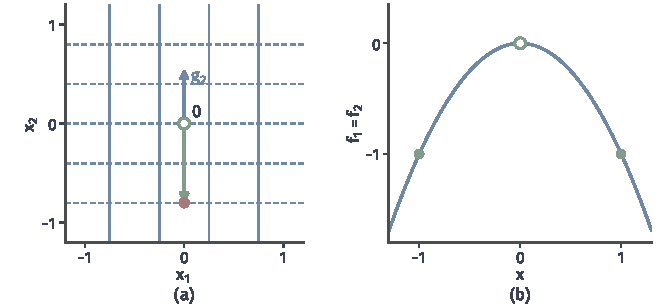
\includegraphics[width=112mm]{figures/05-optimization/07-multiple-criteria-and-nested-optimization/matplotlib/moo-stationary-gap/figure.pdf}
  \caption{Pareto驻定不足以断定最优。(a)式~\eqref{eq:moo-stationary-weak}，竖线是$f_1$的等高线，虚线是$f_2$的等高线；在空心点（原点）处$\bm{g}_1=\bm{0}$，沿绿色箭头$f_1$不变、$f_2$下降，红点支配原点。(b)$f_1=f_2=-x^2$，空心点是驻定点，两个绿点的目标都更小。}
  \label{fig:moo-stationary-gap}
\end{BookInlineFigure}

\paragraph{凸问题中的充分性}
要从驻定走到最优，需要凸性。此时式~\eqref{eq:moo-stationary}的系数$\bm{\theta}$恰好提供了一组权重。

\begin{theorem}[凸问题的驻定点]
\label{thm:moo-stationary-sufficient}
设$\bm{C}=\mathbb{R}^n$，各$f_i$凸且可微，$\bm{x}$满足式~\eqref{eq:moo-stationary}。则$\bm{x}$是$\sum_i\theta_if_i$的全局最小点，因而是全局弱Pareto最优点；若所有$\theta_i>0$，$\bm{x}$是全局Pareto最优点。
\end{theorem}

\begin{proof}
$\sum_i\theta_if_i$是凸函数，其梯度在$\bm{x}$处为零，由第~\ref{chap:optimization}章的一阶条件，$\bm{x}$是它的全局最小点。再由定理~\ref{thm:moo-weighted}得结论。
\end{proof}

式~\eqref{eq:moo-stationary-weak}的原点符合定理的条件，但$\theta_2=0$，所以只能得到弱Pareto最优，这正好和前面看到的现象一致。在例~\eqref{eq:moo-iso}的线段内部，$\bm{\theta}$的两个分量都为正，得到的是Pareto最优。

\subsection{可行方向}
\label{sec:moo-feasible-direction}

候选点若在可行集边界上，只有一部分方向走得动，梯度的凸包不含零也不等于存在可行的共同下降方向。这一小节把判别限制在可行方向上，并调用第~\ref{chap:constrained-optimality}章的约束条件。

\paragraph{问题与记号}
由于$m$已经用来表示目标个数，约束的下标改写为
\[
 \bm{C}=\{\bm{x}:g_j(\bm{x})\leq0,\ j=1,\ldots,q,\ \ h_k(\bm{x})=0,\ k=1,\ldots,p\}.
\]
活动集$A(\bar{\bm{x}})$、切锥$\bm{T}_{\bm{C}}(\bar{\bm{x}})$、线性化锥、LICQ、MFCQ的含义都与第~\ref{chap:constrained-optimality}章相同，只是把不等式的下标换成了$j$，等式的下标换成了$k$。这里的$g_j$是约束函数，加粗的$\bm{g}_i$才是目标的梯度。

\paragraph{切锥上的必要条件}
“能走的方向”由切锥描述，一阶必要条件的形式与单目标的切锥条件相同。

\begin{theorem}[切锥上的必要条件]
\label{thm:moo-tangent-necessary}
设$\bar{\bm{x}}$是局部弱Pareto最优点，各$f_i$在$\bar{\bm{x}}$处可微。则不存在$\bm{d}\in\bm{T}_{\bm{C}}(\bar{\bm{x}})$，使
\begin{equation}
 \langle\nabla f_i(\bar{\bm{x}}),\bm{d}\rangle<0\quad\text{对所有}\ i=1,\ldots,m.
 \label{eq:moo-tangent-descent}
\end{equation}
\end{theorem}

\begin{proof}
设这样的$\bm{d}$存在。由切锥定义，有可行点列$\bm{x}^{(k)}\to\bar{\bm{x}}$与$t_k\downarrow0$，使$(\bm{x}^{(k)}-\bar{\bm{x}})/t_k\to\bm{d}$。Taylor展开并除以$t_k$，
\[
 \frac{f_i(\bm{x}^{(k)})-f_i(\bar{\bm{x}})}{t_k}\to\langle\nabla f_i(\bar{\bm{x}}),\bm{d}\rangle<0.
\]
目标个数有限，所以$k$足够大时，所有$f_i(\bm{x}^{(k)})<f_i(\bar{\bm{x}})$同时成立，与局部弱Pareto最优矛盾。
\end{proof}

\paragraph{目标权重与约束乘子}
切锥不容易计算。约束资格把它换成线性化锥，结论就可以用乘子写出来，形式上是把KKT条件中目标的梯度换成目标梯度的凸组合。

证明不用重新做Farkas那一套，把问题改写成单目标问题即可：引入一个变量$t$代表“所有目标相对当前点的最大变化”，然后要求这个变化不能为负。

\begin{theorem}[多目标KKT必要条件]
\label{thm:moo-kkt-necessary}
设$f_i$、$g_j$、$h_k$在局部弱Pareto最优点$\bar{\bm{x}}$附近连续可微，并且$\bar{\bm{x}}$满足MFCQ。则存在$\bm{\theta}\in\Delta_m$，$\bm{\lambda}\geq\bm{0}$，$\bm{\nu}$，使
\begin{equation}
 \sum_{i=1}^m\theta_i\nabla f_i(\bar{\bm{x}})
 +\sum_{j=1}^q\lambda_j\nabla g_j(\bar{\bm{x}})
 +\sum_{k=1}^p\nu_k\nabla h_k(\bar{\bm{x}})=\bm{0},
 \label{eq:moo-kkt}
\end{equation}
并且$\lambda_jg_j(\bar{\bm{x}})=0$对所有$j$成立。
\end{theorem}

\begin{proof}
考虑变量为$(\bm{x},t)$的单目标问题
\[
 \min_{\bm{x},t}\ t\quad\text{s.t.}\quad
 f_i(\bm{x})-f_i(\bar{\bm{x}})-t\leq0,\ \ \bm{x}\in\bm{C}.
\]

先说明$(\bar{\bm{x}},0)$是它的局部最小点。若$\bm{x}$靠近$\bar{\bm{x}}$，$(\bm{x},t)$可行且$t<0$，则$f_i(\bm{x})<f_i(\bar{\bm{x}})$对所有$i$成立，与局部弱Pareto最优矛盾。

再说明MFCQ在$(\bar{\bm{x}},0)$处成立。设$\bar{\bm{d}}$是原约束的MFCQ方向。增广问题中等式约束的梯度是$(\nabla h_k,0)$，线性无关；取方向$(\bar{\bm{d}},\sigma)$，$\sigma$足够大，则
\[
 \langle\nabla f_i(\bar{\bm{x}}),\bar{\bm{d}}\rangle-\sigma<0\quad\text{对所有}\ i,
\]
其余条件与原约束相同。

由第~\ref{chap:constrained-optimality}章的KKT必要性定理，存在乘子$\bm{\theta}\geq\bm{0}$（对应$f_i-f_i(\bar{\bm{x}})-t\leq0$）、$\bm{\lambda}\geq\bm{0}$与$\bm{\nu}$。对$t$的驻定条件是$1-\sum_i\theta_i=0$，所以$\bm{\theta}\in\Delta_m$；对$\bm{x}$的驻定条件是式~\eqref{eq:moo-kkt}；互补条件来自原约束的互补松弛。
\end{proof}

约束资格不能省。取一元变量，$f_1(x)=f_2(x)=x$，约束$g(x)=x^2\leq0$。可行集只有$\{0\}$，所以$0$是Pareto最优点。但$\nabla f_1=\nabla f_2=1$，$\nabla g(0)=0$，式~\eqref{eq:moo-kkt}左边恒等于$1$。这里MFCQ失败，因为$\langle\nabla g(0),d\rangle=0$，不可能严格小于零。

\paragraph{凸问题中的充分性}
和无约束情形一样，充分性需要凸性，而且权重的符号决定结论的强弱。

\begin{theorem}[凸问题的多目标KKT充分性]
\label{thm:moo-kkt-sufficient}
设$\bm{D}$是包含$\bm{C}$的开凸集，$f_i$、$g_j$在$\bm{D}$上凸且可微，$h_k$仿射。若可行点$\bar{\bm{x}}$满足式~\eqref{eq:moo-kkt}，$\bm{\theta}\in\Delta_m$，$\bm{\lambda}\geq\bm{0}$，且互补松弛成立，则$\bar{\bm{x}}$是$\sum_i\theta_if_i$在$\bm{C}$上的全局最小点，因而是全局弱Pareto最优点；若所有$\theta_i>0$，$\bar{\bm{x}}$是全局Pareto最优点。
\end{theorem}

\begin{proof}
式~\eqref{eq:moo-kkt}与互补松弛正是凸问题$\min_{\bm{C}}\sum_i\theta_if_i$的KKT条件。由第~\ref{chap:constrained-optimality}章的凸问题KKT充分性，$\bar{\bm{x}}$是全局最小点。再由定理~\ref{thm:moo-weighted}得结论。
\end{proof}

这里没有要求约束资格，这与单目标的凸问题相同。必要性要约束资格而不要凸性，充分性要凸性而不要约束资格，两个方向的条件不能互换。

\paragraph{例：无约束判据为什么失效}
在例~\eqref{eq:moo-iso}上加一个约束$g(\bm{x})=x_1+x_2-1/2\leq0$。原来的解集$x_1+x_2=1$整条被挡在可行集外面，新的候选应该在边界上。取$\bar{\bm{x}}=(1/4,1/4)$，
\[
 \bm{g}_1=\bar{\bm{x}}-\bm{a}=(-3/4,1/4),\qquad\bm{g}_2=\bar{\bm{x}}-\bm{b}=(1/4,-3/4).
\]

这两个梯度的凸包不含零。取$\bm{\theta}=(1/2,1/2)$得到其中最短的组合
\[
 \bar{\bm{g}}=(-1/4,-1/4).
\]
如果套用无约束判据，就会以为$\bar{\bm{x}}$不是驻定点。可是下降方向$-\bar{\bm{g}}=(1/4,1/4)$走出了可行集，这一步根本走不了。

加上约束的乘子就对了。由式~\eqref{eq:moo-kkt}，$\nabla g=(1,1)$，
\[
 \tfrac12\bm{g}_1+\tfrac12\bm{g}_2+\lambda(1,1)=\bm{0},
\]
解得$\lambda=1/4\geq0$。$\bar{\bm{x}}$在边界上，互补松弛成立，问题是凸的，权重全正，由定理~\ref{thm:moo-kkt-sufficient}，$\bar{\bm{x}}$是全局Pareto最优点。

更一般地，式~\eqref{eq:moo-kkt}对可行点$\bm{x}$写出来是$\bm{x}=(\theta-\lambda,1-\theta-\lambda)$，其中$\bm{\theta}=(\theta,1-\theta)$。边界条件$x_1+x_2=1/2$给出$\lambda=1/4$，所以约束问题的驻定点是
\begin{equation}
 \bm{x}=\bigl(\theta-\tfrac14,\ \tfrac34-\theta\bigr),\qquad 0\leq\theta\leq1.
 \label{eq:moo-feasible-set}
\end{equation}

代入目标，前沿是$\bigl((1-\theta)^2+\tfrac1{16},\ \theta^2+\tfrac1{16}\bigr)$，恰是原前沿沿两个方向平移$1/16$。图~\ref{fig:moo-feasible-pareto}把解集和前沿画了出来。

\begin{BookInlineFigure}
  \centering
  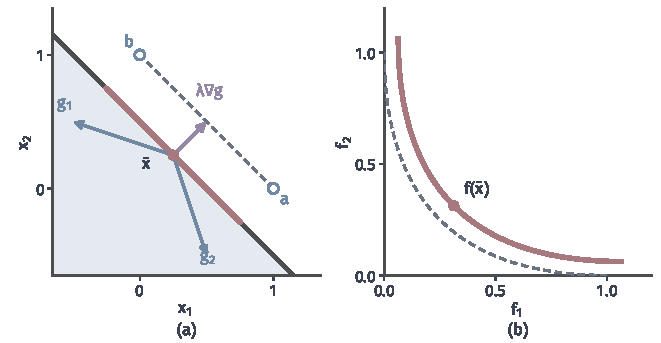
\includegraphics[width=112mm]{figures/05-optimization/07-multiple-criteria-and-nested-optimization/matplotlib/moo-feasible-pareto/figure.pdf}
  \caption{加上半平面约束$x_1+x_2\leq1/2$后的例子。(a)深灰粗线是活动约束，红色线段是约束下的解集（式~\eqref{eq:moo-feasible-set}），虚线是原来的解集；在$\bar{\bm{x}}=(1/4,1/4)$处，$\bm{g}_1,\bm{g}_2$的中点被紫色的$\lambda\nabla g$抵消。(b)红色曲线是约束下的前沿，虚线是原前沿，红点是$\bm{f}(\bar{\bm{x}})=(5/16,5/16)$。}
  \label{fig:moo-feasible-pareto}
\end{BookInlineFigure}

端点$\theta=0,1$的权重有零，但此时分别是$f_2$、$f_1$在可行集上的唯一最小点，由定理~\ref{thm:moo-weighted}的第~3条仍是Pareto最优点。这说明定理~\ref{thm:moo-kkt-sufficient}中“全正”只是充分条件，端点要单独检查。

\section{多梯度下降}
\label{sec:moo-mgda}

第~\ref{sec:moo-common-descent}节的判别给出了一个方向：梯度凸包中离原点最近的点。这一节把它变成迭代。问题是：怎样在几个目标的梯度之间取折中，才能保证一步之后每个目标都不变差？

由此得到的方法称为\term{多梯度下降算法}（multiple-gradient descent algorithm，MGDA）。它不需要事先给定偏好，权重是每一步按当前的几何现算的，这一点和固定加权和不同。

\subsection{最小范数组合}
\label{sec:moo-min-norm}

\paragraph{主要思想}
最简单的想法是把各目标的梯度平均一下，然后沿反方向走。看一个具体的数据：
\[
 \bm{g}_1=(10,1),\qquad\bm{g}_2=(-1,1).
\]
平均后得$(4.5,1)$，方向是$\bm{d}=(-4.5,-1)$。检查第二个目标的方向导数：
\[
 \langle\bm{g}_2,\bm{d}\rangle=4.5-1=3.5>0.
\]
$f_2$反而上升。梯度长度悬殊时，长的那个梯度支配了平均，短的那个目标被牺牲了。

\begin{BookInlineFigure}
  \centering
  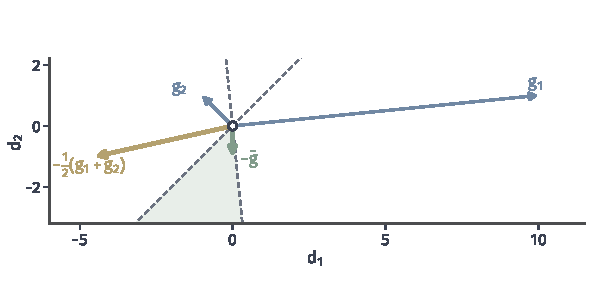
\includegraphics[width=100mm]{figures/05-optimization/07-multiple-criteria-and-nested-optimization/matplotlib/moo-average-vs-minnorm/figure.pdf}
  \caption{平均方向与最小范数方向，$\bm{g}_1=(10,1)$，$\bm{g}_2=(-1,1)$。两条灰色虚线分别垂直于两个梯度，浅绿楔形是共同下降方向。黄色箭头是平均梯度的反方向，落在楔形外；绿色箭头是$-\bar{\bm{g}}=(0,-1)$，落在楔形内。}
  \label{fig:moo-average-vs-minnorm}
\end{BookInlineFigure}

要保证每个目标都下降，应当转而问：在所有梯度的加权平均中，哪一个最短？记
\begin{equation}
 \bm{\theta}^\star\in\argmin_{\bm{\theta}\in\Delta_m}\ \frac12\Bigl\lVert\sum_{i=1}^m\theta_i\bm{g}_i\Bigr\rVert_2^2,
 \qquad
 \bar{\bm{g}}=\sum_{i=1}^m\theta_i^\star\bm{g}_i,
 \label{eq:moo-min-norm}
\end{equation}
并取方向$\bm{d}=-\bar{\bm{g}}$。式~\eqref{eq:moo-min-norm}的权重子问题在单纯形上最小化一个凸二次函数。$\bar{\bm{g}}$是原点在凸包上的投影，所以唯一，而$\bm{\theta}^\star$不一定唯一。

在上面的数据上，后面的式~\eqref{eq:moo-theta-two}给出$\theta_1^\star=1/11$，于是$\bar{\bm{g}}=(0,1)$，方向$(0,-1)$落在共同下降的楔形内，见图~\ref{fig:moo-average-vs-minnorm}。两个方向导数都等于$-1$。

\begin{lemma}[最小范数组合的下降性质]
\label{lem:moo-min-norm}
对式~\eqref{eq:moo-min-norm}定义的$\bar{\bm{g}}$，
\begin{equation}
 \langle\bm{g}_i,-\bar{\bm{g}}\rangle\leq-\lVert\bar{\bm{g}}\rVert_2^2\quad\text{对所有}\ i=1,\ldots,m.
 \label{eq:moo-min-norm-descent}
\end{equation}
并且$\bar{\bm{g}}=\bm{0}$当且仅当$\bm{x}$是无约束的Pareto驻定点。
\end{lemma}

\begin{proof}
不等式已在引理~\ref{lem:moo-gordan}的证明中得到，投影性质给出
\[
 \langle\bm{g}_i,\bar{\bm{g}}\rangle\geq\lVert\bar{\bm{g}}\rVert_2^2,
\]
这对$\bar{\bm{g}}=\bm{0}$也成立。第二句是Pareto驻定的定义：$\bm{0}$在凸包中，当且仅当它到凸包的最短距离为零。
\end{proof}

式~\eqref{eq:moo-min-norm-descent}是整个方法的关键：只要$\bar{\bm{g}}\neq\bm{0}$，每个目标的方向导数都不大于$-\lVert\bar{\bm{g}}\rVert_2^2$，都确实在下降，而且下降速度有统一的下界。

\paragraph{两个目标的闭式解}
$m=2$时，令$\bm{\theta}=(\theta,1-\theta)$，$\bm{g}_1\neq\bm{g}_2$。子问题是一元二次函数：
\[
 \phi(\theta)=\lVert\theta\bm{g}_1+(1-\theta)\bm{g}_2\rVert_2^2=\lVert\bm{g}_2+\theta(\bm{g}_1-\bm{g}_2)\rVert_2^2.
\]
求导令其为零，得到无约束的最小点$\langle\bm{g}_2,\bm{g}_2-\bm{g}_1\rangle/\lVert\bm{g}_1-\bm{g}_2\rVert_2^2$。把它截断到$[0,1]$，由于$\phi$是凸的一元二次函数，截断后仍是区间上的最小点：
\begin{equation}
 \theta^\star=\min\Bigl\{1,\ \max\Bigl\{0,\ \frac{\langle\bm{g}_2,\bm{g}_2-\bm{g}_1\rangle}{\lVert\bm{g}_1-\bm{g}_2\rVert_2^2}\Bigr\}\Bigr\}.
 \label{eq:moo-theta-two}
\end{equation}
若$\bm{g}_1=\bm{g}_2$，任取$\theta$都得到同一个$\bar{\bm{g}}$。

图~\ref{fig:moo-min-norm}是三种情形。(a)垂足落在线段内部，$0<\theta^\star<1$，此时式~\eqref{eq:moo-min-norm-descent}对两个目标都取等号，两个目标下降速度相同。(b)垂足落在线段之外，截断后$\bar{\bm{g}}$就是较短的梯度，方向只对那一个目标是最陡的，另一个目标下降得更快。(c)原点在线段上，$\bar{\bm{g}}=\bm{0}$，停止。

\begin{BookInlineFigure}
  \centering
  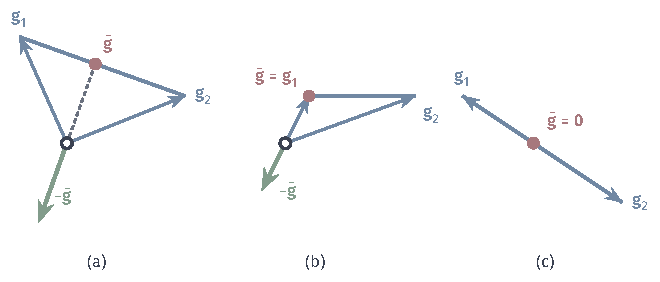
\includegraphics[width=111.8mm]{figures/05-optimization/07-multiple-criteria-and-nested-optimization/tikz/moo-min-norm/figure.pdf}
  \caption{两个梯度的最小范数组合。蓝色线段是凸包，红点是$\bar{\bm{g}}$，绿色箭头是$-\bar{\bm{g}}$，空心点是原点。(a)垂足在线段内部。(b)垂足在线段外，截断到较短的梯度$\bm{g}_1$。(c)原点在线段上，点是Pareto驻定的，没有更新方向。}
  \label{fig:moo-min-norm}
\end{BookInlineFigure}

\paragraph{方向的最优性}
最小范数这个构造还可以从另一面看：它正好是一个“保最差目标”的方向问题的解。假设只看一阶模型，希望下降最少的目标也尽量下降，同时用$\frac12\lVert\bm{d}\rVert_2^2$防止步子过大。

\begin{theorem}[最坏目标的最陡方向]
\label{thm:moo-steepest}
问题
\begin{equation}
 \min_{\bm{d}\in\mathbb{R}^n}\ \max_{1\leq i\leq m}\langle\bm{g}_i,\bm{d}\rangle+\frac12\lVert\bm{d}\rVert_2^2
 \label{eq:moo-steepest}
\end{equation}
的唯一解是$\bm{d}=-\bar{\bm{g}}$，最优值是$-\frac12\lVert\bar{\bm{g}}\rVert_2^2$。
\end{theorem}

\begin{proof}
目标是凸函数加强凸函数，解唯一。对任意$\bm{d}$，最大值不小于凸组合，所以
\[
 \max_i\langle\bm{g}_i,\bm{d}\rangle+\tfrac12\lVert\bm{d}\rVert_2^2
 \geq\langle\bar{\bm{g}},\bm{d}\rangle+\tfrac12\lVert\bm{d}\rVert_2^2.
\]
右端关于$\bm{d}$的最小值在$\bm{d}=-\bar{\bm{g}}$取到，所以
\[
 \max_i\langle\bm{g}_i,\bm{d}\rangle+\tfrac12\lVert\bm{d}\rVert_2^2
 \geq-\tfrac12\lVert\bar{\bm{g}}\rVert_2^2.
\]

反过来，取$\bm{d}=-\bar{\bm{g}}$，由式~\eqref{eq:moo-min-norm-descent}，最大值不超过$-\lVert\bar{\bm{g}}\rVert_2^2$，目标不超过$-\frac12\lVert\bar{\bm{g}}\rVert_2^2$。两边合起来取等，$-\bar{\bm{g}}$是解。
\end{proof}

\paragraph{权重的含义}
$\bm{\theta}^\star$看起来也是一组权重，但它与加权和的权重$\bm{w}$职责不同，见表~\ref{tab:moo-weights}。$\bm{w}$是决策者给定的，整个求解过程中不变，表达的是偏好。$\bm{\theta}^\star$是算法每一步根据当前梯度算出来的，表达的是当前的几何。

\begin{BookInlineTable}
  \centering
  \caption{固定加权与多梯度下降中的权重。}
  \label{tab:moo-weights}
  \begin{tabular}{@{}lll@{}}
    \toprule
     & 加权和的$\bm{w}$ & 多梯度下降的$\bm{\theta}^\star$\\
    \midrule
    来源 & 使用者事先给定 & 每步由梯度算出\\
    迭代中 & 固定 & 随$\bm{x}$变化\\
    单个目标 & 可能上升 & 不上升（配合步长）\\
    终点 & 该偏好下的解 & 取决于起点的一个驻定点\\
    \bottomrule
  \end{tabular}
\end{BookInlineTable}

要注意$\bm{\theta}^\star$不是尺度无关的。把上面的$f_1$除以$10$，$\bm{g}_1$变成$(1,0.1)$，由式~\eqref{eq:moo-theta-two}算得$\theta^\star\approx0.603$，$\bar{\bm{g}}\approx(0.206,0.457)$，方向和原来的$(0,1)$不同。所以第~\ref{sec:moo-scale}节的提醒在这里同样适用：梯度长度悬殊的问题，先要说明目标的尺度。

$m>2$时，令$\bm{G}$是$m\times m$矩阵，元素为$\bm{G}_{i,j}=\langle\bm{g}_i,\bm{g}_j\rangle$，子问题就是在单纯形上最小化$\frac12\bm{\theta}^\top\bm{G}\bm{\theta}$。第~\ref{chap:quadratic-conic-programming}章的二次规划方法和第~\ref{chap:feasible-iterations}章的Frank--Wolfe方法都能解它。单纯形的规模只有$m$，主要开销在于计算$m$个梯度和$\bm{G}$的$O(m^2n)$次运算。

\subsection{共同步长}
\label{sec:moo-common-step}

有了方向，还要决定走多远。若沿各自的梯度分别走一步，再把得到的位置取平均，效果等同于沿平均梯度走一步，前面已经看到这可能让某个目标上升。所以这一小节要为所有目标选一个共同的步长，并检查每一个目标的下降。

\paragraph{多目标的充分下降}
把单目标的回溯规则（第~\ref{chap:smooth-foundations}章）推广：一个步长$\alpha>0$只有在所有目标都达到下面的下降量时才被接受，
\begin{equation}
 f_i(\bm{x}-\alpha\bar{\bm{g}})\leq f_i(\bm{x})-c\,\alpha\lVert\bar{\bm{g}}\rVert_2^2\quad\text{对所有}\ i,
 \label{eq:moo-armijo}
\end{equation}
其中$c\in(0,1)$，常取$c=1/2$。回溯时从$\alpha=1$开始，不满足就乘以$\beta\in(0,1)$，这里取$\beta=1/2$。

为什么步长一定找得到？设每个$\nabla f_i$是$L_i$-Lipschitz的，记$L_{\max}=\max_iL_i$。由下降引理（第~\ref{chap:smooth-foundations}章）和式~\eqref{eq:moo-min-norm-descent}，
\[
 f_i(\bm{x}-\alpha\bar{\bm{g}})
 \leq f_i(\bm{x})+\alpha\langle\bm{g}_i,-\bar{\bm{g}}\rangle+\frac{L_i\alpha^2}{2}\lVert\bar{\bm{g}}\rVert_2^2
 \leq f_i(\bm{x})-\alpha\Bigl(1-\frac{L_i\alpha}{2}\Bigr)\lVert\bar{\bm{g}}\rVert_2^2.
\]
所以当$\alpha\leq1/L_{\max}$时，括号不小于$1/2$，式~\eqref{eq:moo-armijo}在$c=1/2$时成立。

从这里也看得出共同步长的代价：步长受曲率最大的那个目标限制，$L_{\max}$很大时所有目标都得小步前进。

\paragraph{计算过程}
下面在一个病态的例子上走三轮。目标的第一项是第~\ref{chap:smooth-foundations}章贯穿使用的二次函数，第二项把点拉向$(4,3)$：
\begin{equation}
 f_1(\bm{x})=\frac12(x_1^2+9x_2^2),\qquad
 f_2(\bm{x})=\frac12\bigl[(x_1-4)^2+(x_2-3)^2\bigr].
 \label{eq:moo-mgda-example}
\end{equation}

\needspace{6\baselineskip}
\paragraph{变量}
\begin{itemize}
 \item 迭代点$\bm{x}^{(t)}\in\mathbb{R}^n$，各目标的值$f_i(\bm{x}^{(t)})$；
 \item 梯度$\bm{g}_i^{(t)}=\nabla f_i(\bm{x}^{(t)})$，$i=1,\ldots,m$；
 \item 组合系数$\bm{\theta}^{(t)}\in\Delta_m$，组合梯度$\bar{\bm{g}}^{(t)}$；
 \item 步长$\alpha^{(t)}$，常数$c$、$\beta$，容差$\epsilon$。
\end{itemize}

\paragraph{初始化}
给定起点$\bm{x}^{(0)}$和容差$\epsilon$。例中取$\bm{x}^{(0)}=(1,1)$，$c=\beta=1/2$，此时目标值为
\[
 \bm{f}(\bm{x}^{(0)})=(5,\ 6.5).
\]

\paragraph{每轮更新}
对$t=0,1,\ldots$重复下列步骤，直到$\lVert\bar{\bm{g}}^{(t)}\rVert_2\leq\epsilon$。

\begin{enumerate}
 \item 计算各目标的梯度。例中第一轮
 \[
  \bm{g}_1^{(0)}=(1,9),\qquad\bm{g}_2^{(0)}=(-3,-2).
 \]

 \item 由式~\eqref{eq:moo-min-norm}求$\bm{\theta}^{(t)}$与$\bar{\bm{g}}^{(t)}$，两个目标时用式~\eqref{eq:moo-theta-two}。例中第一轮
 \[
  \theta^{(0)}=\frac{34}{137}\approx0.2482,\qquad
  \bar{\bm{g}}^{(0)}\approx(-2.0073,\ 0.7299),
 \]
 并且$\lVert\bar{\bm{g}}^{(0)}\rVert_2^2\approx4.5620$。

 \item 回溯求步长：从$\alpha=1$开始，检查式~\eqref{eq:moo-armijo}是否对每一个目标成立。例中$\alpha=1$的试探点是$(3.0073,0.2701)$，$f_1\approx4.8501$，而要求不超过$5-\frac12\times4.5620\approx2.7190$，被拒绝。$\alpha=1/2$的试探点满足两个目标的要求：
 \[
  f_1\approx3.8220\leq3.8595,\qquad f_2\approx4.7892\leq5.3595.
 \]

 \item 沿$-\bar{\bm{g}}^{(t)}$走一步，更新为
 \begin{equation}
  \bm{x}^{(t+1)}=\bm{x}^{(t)}-\alpha^{(t)}\bar{\bm{g}}^{(t)}.
  \label{eq:moo-mgda-update}
 \end{equation}
 例中第一轮
 \[
  \bm{x}^{(1)}\approx(2.0036,\ 0.6350),\qquad
  \bm{f}(\bm{x}^{(1)})\approx(3.8220,\ 4.7892).
 \]
\end{enumerate}

第二轮的梯度是
\[
 \bm{g}_1^{(1)}\approx(2.0036,\ 5.7153),\qquad
 \bm{g}_2^{(1)}\approx(-1.9964,\ -2.3650).
\]
由此算得
\[
 \theta^{(1)}\approx0.3333,\quad
 \bar{\bm{g}}^{(1)}\approx(-0.6631,\ 0.3283),\quad
 \lVert\bar{\bm{g}}^{(1)}\rVert_2^2\approx0.5475.
\]
$\alpha=1$和$\alpha=1/2$都因$f_1$不满足式~\eqref{eq:moo-armijo}被拒绝，$\alpha=1/4$被接受，得到
\[
 \bm{x}^{(2)}\approx(2.1694,\ 0.5530),\qquad
 \bm{f}(\bm{x}^{(2)})\approx(3.7292,\ 4.6695).
\]

第三轮的梯度是
\[
 \bm{g}_1^{(2)}\approx(2.1694,\ 4.9767),\qquad
 \bm{g}_2^{(2)}\approx(-1.8306,\ -2.4470).
\]
算得
\[
 \theta^{(2)}\approx0.3584,\quad
 \bar{\bm{g}}^{(2)}\approx(-0.3969,\ 0.2138),\quad
 \lVert\bar{\bm{g}}^{(2)}\rVert_2^2\approx0.2032.
\]
同样$\alpha=1/4$被接受，
\[
 \bm{x}^{(3)}\approx(2.2687,\ 0.4995),\qquad
 \bm{f}(\bm{x}^{(3)})\approx(3.6962,\ 4.6250).
\]
可以看到，两个目标每一轮都严格下降，$\theta^{(t)}$在逐轮变化。

最终得到$\bm{x}^\star\approx(2.3933,0.4260)$，目标值约为$(3.6808,4.6034)$，$\bar{\bm{g}}$的范数已到舍入误差量级。这一点的$\theta^\star\approx0.4017$，用它作权重，第~\ref{sec:moo-weighted}节的加权和在这一点取到最优。

\begin{BookInlineFigure}
  \centering
  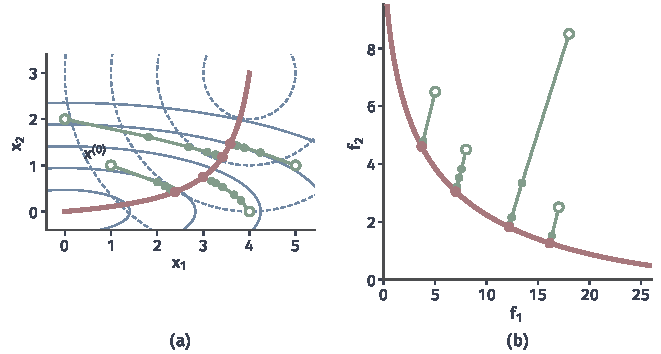
\includegraphics[width=112mm]{figures/05-optimization/07-multiple-criteria-and-nested-optimization/matplotlib/moo-mgda-path/figure.pdf}
  \caption{多梯度下降在例~\eqref{eq:moo-mgda-example}上的路径。(a)决策平面，实线与虚线分别是$f_1,f_2$的等高线，红色曲线是Pareto解集，绿线是四个起点（空心点）的路径，小点是前五步，红点是终点。(b)同一批路径在目标平面上的像，红色曲线是Pareto前沿。不同起点落到前沿的不同位置。}
  \label{fig:moo-mgda-path}
\end{BookInlineFigure}

\paragraph{收敛性}
图~\ref{fig:moo-mgda-path}显示，路径都在目标平面上朝左下方走，最后落到前沿上，不同起点落到不同位置。下面的定理说明能够保证的是什么。

\begin{theorem}[多梯度下降的收敛]
\label{thm:moo-mgda-convergence}
设每个$f_i$有下界$f_i^{\mathrm{low}}$，$\nabla f_i$是$L_i$-Lipschitz的，记$L_{\max}=\max_iL_i$。设迭代满足式~\eqref{eq:moo-armijo}，且$\alpha^{(t)}\geq\alpha_{\min}>0$。则对任意目标$i$和任意$T\geq1$，
\begin{equation}
 \min_{0\leq t<T}\lVert\bar{\bm{g}}^{(t)}\rVert_2^2
 \leq\frac{f_i(\bm{x}^{(0)})-f_i^{\mathrm{low}}}{c\,\alpha_{\min}T}.
 \label{eq:moo-mgda-rate}
\end{equation}
并且序列的每个极限点都是Pareto驻定点。固定步长$\alpha=1/L_{\max}$，$c=1/2$时满足条件，式~\eqref{eq:moo-mgda-rate}的右端为$2L_{\max}(f_i(\bm{x}^{(0)})-f_i^{\mathrm{low}})/T$。
\end{theorem}

\begin{proof}
由式~\eqref{eq:moo-armijo}，对每个$t$，
\[
 f_i(\bm{x}^{(t+1)})\leq f_i(\bm{x}^{(t)})-c\,\alpha_{\min}\lVert\bar{\bm{g}}^{(t)}\rVert_2^2.
\]
对$t=0,\ldots,T-1$求和，利用$f_i(\bm{x}^{(T)})\geq f_i^{\mathrm{low}}$，得到
\[
 c\,\alpha_{\min}\sum_{t=0}^{T-1}\lVert\bar{\bm{g}}^{(t)}\rVert_2^2\leq f_i(\bm{x}^{(0)})-f_i^{\mathrm{low}}.
\]
最小项不超过平均值，即得式~\eqref{eq:moo-mgda-rate}。这一和式也说明$\lVert\bar{\bm{g}}^{(t)}\rVert_2\to0$。

记$\varphi(\bm{x})$为点$\bm{x}$处的$\lVert\bar{\bm{g}}\rVert_2$。对任意$\bm{x},\bm{y}$，设$\bm{\theta}$是$\bm{y}$处的最优系数，
\[
 \varphi(\bm{x})\leq\Bigl\lVert\sum_i\theta_i\nabla f_i(\bm{x})\Bigr\rVert_2
 \leq\varphi(\bm{y})+L_{\max}\lVert\bm{x}-\bm{y}\rVert_2.
\]
交换$\bm{x},\bm{y}$，两式合起来给出
\[
 \lvert\varphi(\bm{x})-\varphi(\bm{y})\rvert\leq L_{\max}\lVert\bm{x}-\bm{y}\rVert_2,
\]
所以$\varphi$连续。沿收敛子列取极限，极限点处$\varphi=0$，由引理~\ref{lem:moo-min-norm}它是Pareto驻定点。

固定步长的情形由式~\eqref{eq:moo-armijo}之后的不等式给出。
\end{proof}

定理的结论是$\lVert\bar{\bm{g}}\rVert_2$趋于零，也就是逼近Pareto驻定。根据第~\ref{sec:moo-common-descent}节，这不等于全局Pareto最优；凸问题中，再加上极限处权重全正，才能推到Pareto最优。回溯时取$\alpha_{\min}=\min\{1,\beta/L_{\max}\}$即可满足定理的条件，因为一旦$\alpha\leq1/L_{\max}$就会被接受。

\paragraph{与固定加权的对比}
图~\ref{fig:moo-mgda-curves}比较了从$(4,0)$出发的两种迭代。这一点的目标值是$(8,4.5)$。固定权重$(1/2,1/2)$的梯度法（黄色）走向该偏好下的解$(2.41,5.64)$，$f_1$降了很多，但$f_2$从$4.5$升到了$5.64$。多梯度下降（绿色）停在$(6.99,3.04)$，两个目标都比起点好。

这两个结果没有谁对谁错。前者忠实地执行了“两项同样重要”的偏好，后者忠实地执行了“不让任何一项变差”的要求。一次运行得到的都只是前沿上的一个点。

\begin{BookInlineFigure}
  \centering
  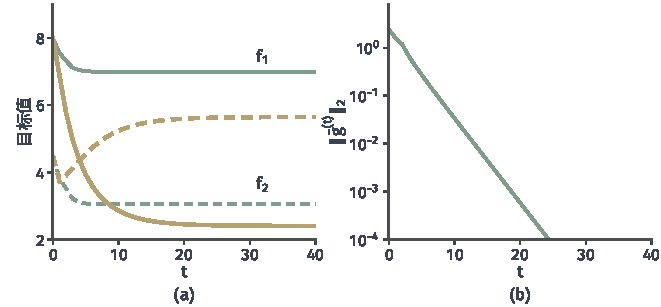
\includegraphics[width=112mm]{figures/05-optimization/07-multiple-criteria-and-nested-optimization/matplotlib/moo-mgda-curves/figure.pdf}
  \caption{从$(4,0)$出发的迭代，例~\eqref{eq:moo-mgda-example}。(a)实线是$f_1$，虚线是$f_2$，绿色是多梯度下降，黄色是固定权重$(1/2,1/2)$、步长$1/L$的梯度法，后者使$f_2$上升。(b)多梯度下降的$\lVert\bar{\bm{g}}^{(t)}\rVert_2$，纵轴为对数。}
  \label{fig:moo-mgda-curves}
\end{BookInlineFigure}

\paragraph{有约束时}
可行集$\bm{C}$是闭凸集时，把式~\eqref{eq:moo-steepest}限制到可行方向上：
\begin{equation}
 \bm{d}^{(t)}\in\argmin_{\bm{x}^{(t)}+\bm{d}\in\bm{C}}\ \max_i\langle\bm{g}_i^{(t)},\bm{d}\rangle+\frac12\lVert\bm{d}\rVert_2^2.
 \label{eq:moo-feasible-direction}
\end{equation}
$\bm{d}=\bm{0}$是可行的，目标值是$0$。由强凸性解唯一，所以$\bm{d}^{(t)}\neq\bm{0}$时最优值严格小于零，$\max_i\langle\bm{g}_i^{(t)},\bm{d}^{(t)}\rangle<0$，$\bm{d}^{(t)}$是共同下降方向。由$\bm{C}$凸，$\bm{x}^{(t)}+\alpha\bm{d}^{(t)}$在$\alpha\in(0,1]$时可行，沿它做共同步长的回溯即可。

反过来，若存在可行点$\bm{x}^{(t)}+\bm{v}$使$\langle\bm{g}_i^{(t)},\bm{v}\rangle<0$对所有$i$成立，取足够小的$\tau>0$，方向$\tau\bm{v}$的目标值就小于零，于是$\bm{d}=\bm{0}$不是解。所以$\bm{d}^{(t)}=\bm{0}$说明从当前点沿可行集内的方向不存在共同下降，这对应第~\ref{sec:moo-feasible-direction}节的驻定条件。$\bm{C}$是多面体时，式~\eqref{eq:moo-feasible-direction}可以写成一个二次规划。

一次多梯度下降通常只给出前沿上的一个点。要得到一组候选，就要进入下一节。

\section{前沿的计算}
\label{sec:moo-front-computation}

决策者常常要先看到各种取舍，再做决定。这就要求算出一组候选，而不是一个点。单次标量化或一次多梯度下降都只给出前沿上的一点，所以要么反复求解，要么同时维护多个候选。本节分别讨论这两条路：由偏好参数驱动的重复求解，和由支配关系驱动的群体搜索。

\subsection{参数扫描}
\label{sec:moo-scan}

把权重、阈值或参考点变化一遍，每次解一个单目标问题，能否得到一组分布合理的候选？这一小节要说明，参数均匀并不等于前沿均匀，并给出按空缺补充求解的办法。

\paragraph{均匀的参数不等于均匀的前沿}
在例~\eqref{eq:moo-iso}上，由式~\eqref{eq:moo-iso-weighted}，取$w=0,1/4,1/2,3/4,1$，得到前沿上的五个点
\[
 (1,0),\quad(0.5625,0.0625),\quad(0.25,0.25),\quad(0.0625,0.5625),\quad(0,1).
\]
相邻两点的距离依次约为$0.442,0.364,0.364,0.442$，不算均匀，但差得不多。

如果两个目标的尺度悬殊，差别就大了。例~\eqref{eq:moo-mgda-example}的加权和有显式解，由$w\bm{g}_1+(1-w)\bm{g}_2=\bm{0}$逐分量解出
\begin{equation}
 \bm{x}(w)=\Bigl(4(1-w),\ \frac{3(1-w)}{8w+1}\Bigr).
 \label{eq:moo-mgda-weighted}
\end{equation}
图~\ref{fig:moo-scan-gaps}(a)是$11$个均匀的$w$所对应的点，点都挤在左上方，右下方有一个大空缺。按目标范围归一化后，相邻点间距最大约为$0.665$，最小约为$0.089$。

\begin{BookInlineFigure}
  \centering
  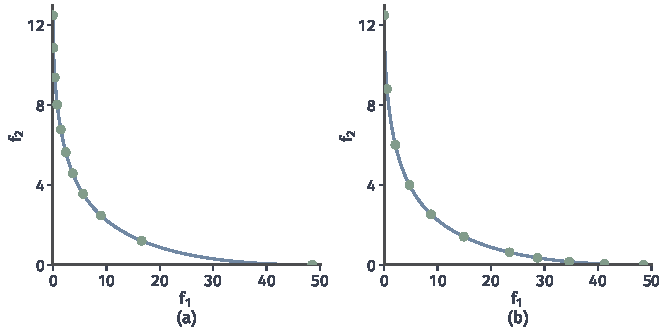
\includegraphics[width=112mm]{figures/05-optimization/07-multiple-criteria-and-nested-optimization/matplotlib/moo-scan-gaps/figure.pdf}
  \caption{例~\eqref{eq:moo-mgda-example}前沿上的$11$个候选。(a)$w$在$[0,1]$上均匀取值，点集中在左上方。(b)按最大空缺逐次补点，权重取空缺两端连线的法向。两图的端点相同。}
  \label{fig:moo-scan-gaps}
\end{BookInlineFigure}

\paragraph{按空缺补点}
既然均匀的参数靠不住，就让已经算出的点来决定下一个参数。对凸前沿，下面的过程很自然。

先用两个端点权重算出两端的点。然后反复做这样一步：找出归一化后间距最大的相邻两点$\bm{p},\bm{q}$，取这两点连线的法向作为新的权重，
\begin{equation}
 w=\frac{\lvert q_2-p_2\rvert}{\lvert q_2-p_2\rvert+\lvert q_1-p_1\rvert},
 \label{eq:moo-chord-weight}
\end{equation}
求解相应的加权和，把新点插进去。新权重下，支撑线与连线平行，解是这段前沿上离连线最远的点。若解不比$\bm{p},\bm{q}$的连线更靠左下，说明这一段已经没有新的支撑点，把这段标记为完成。

在例~\eqref{eq:moo-iso}上走几步。两端是$(0,1)$和$(1,0)$，由式~\eqref{eq:moo-chord-weight}得$w=1/2$，由式~\eqref{eq:moo-iso-weighted}得新点$(1/4,1/4)$。

在$(0,1)$与$(1/4,1/4)$之间，两个差值是$3/4$和$1/4$，权重为
\[
 w=\frac{3/4}{3/4+1/4}=\frac34,
\]
新点是$(1/16,9/16)$。在$(1/4,1/4)$与$(1,0)$之间，同理$w=1/4$，新点是$(9/16,1/16)$。五个点到此与均匀权重的结果相同，继续补点时，算法开始根据实际空缺分配求解次数。

在例~\eqref{eq:moo-mgda-example}上，按这种做法得到图~\ref{fig:moo-scan-gaps}(b)，归一化间距的最大值降到约$0.296$，最小值约为$0.111$，同样$11$次求解分布均匀得多。这里的选取规则只用到已算出的点，但法向的含义依赖目标尺度，所以要先说明归一化的参考范围。

\paragraph{用邻近问题的解作初值}
相邻参数的解通常相隔不远，这启发了用上一个解作下一个问题的初值，称为\term{热启动}（warm start）。图~\ref{fig:moo-warm-start}比较了两种做法：用梯度法解$39$个加权子问题，步长取该子问题的$1/L$，梯度范数降到$10^{-3}$为止。

\begin{BookInlineFigure}
  \centering
  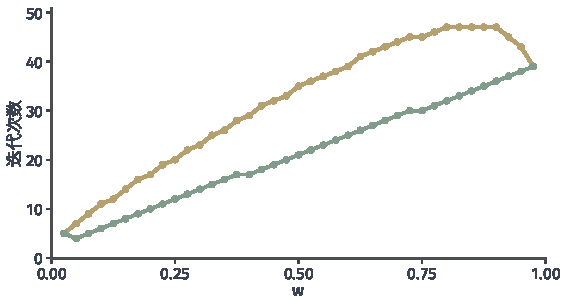
\includegraphics[width=96mm]{figures/05-optimization/07-multiple-criteria-and-nested-optimization/matplotlib/moo-warm-start/figure.pdf}
  \caption{例~\eqref{eq:moo-mgda-example}的$39$个加权子问题所用的梯度法迭代次数，$w$每步增加$0.025$。黄线是每次从$(0,2)$冷启动，共$1232$步；绿线是从上一个解热启动，共$826$步。}
  \label{fig:moo-warm-start}
\end{BookInlineFigure}

总迭代次数从$1232$降到$826$。线性收敛的方法从更好的初值出发，节省的是迭代次数对数中的一项，收敛速率本身不变，所以这里只节省三分之一左右，高精度要求下比例还会更小。

\paragraph{保存非支配候选}
扫描得到的点不一定都有用：求解可能不精确，并列解可能只是弱Pareto最优点。所以要维护一个\term{非支配存档}（non-dominated archive）。新点进来时，若被存档中的点支配就丢弃；否则把它支配的旧点删掉，再加入存档。

按$A,E,B,F,C,D$的顺序把式~\eqref{eq:moo-candidates}中的候选送入存档。$A$进入；$E$与$A$不可比，进入；$B$支配$E$，把$E$换成$B$；$F$与已有的点不可比，进入；$C$也进入；$D$支配$F$，把$F$换成$D$。最后得到$\{A,B,C,D\}$。

\paragraph{可达性的限制仍然存在}
无论参数取得多细，每种标量化能到达的点不会变多。图~\ref{fig:moo-scan-compare}在带凹陷的前沿上各取九个均匀的参数。加权和在$w\geq0.7$的三次求解全落到端点，凹陷段里一个点也没有，点从$(0.577,0.183)$直接跳到$(0.206,0.633)$。阈值约束和加权Chebyshev都把点放进了凹陷。

\begin{BookInlineFigure}
  \centering
  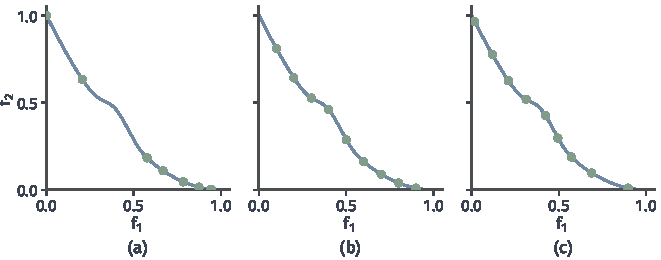
\includegraphics[width=112mm]{figures/05-optimization/07-multiple-criteria-and-nested-optimization/matplotlib/moo-scan-compare/figure.pdf}
  \caption{带凹陷的前沿上三种标量化的扫描，每种取九个均匀参数。(a)加权和，$w=0.1,\ldots,0.9$，$w\geq0.7$的三点重合在左端。(b)阈值约束，$\tau=0.1,\ldots,0.9$。(c)加权Chebyshev，$\bm{z}=(-0.1,-0.1)$，$\bm{w}=(w,1-w)$。}
  \label{fig:moo-scan-compare}
\end{BookInlineFigure}

所以，在非凸前沿上，要用阈值约束或加权Chebyshev来做扫描，并且每次求解都要检查是否达到全局最优。若子问题只解到局部最优，定理~\ref{thm:moo-threshold}和定理~\ref{thm:moo-chebyshev}的保证都不再适用。

\subsection{非支配排序}
\label{sec:moo-nsga}

参数扫描每次只优化一个点。能不能让一批候选同时朝前沿移动，并在前沿上散开？这一小节以NSGA-II为例，说明怎样把第~\ref{chap:random-search}章的种群搜索改造成服务前沿近似的算法。

\paragraph{主要思想}
\term{NSGA-II}（non-dominated sorting genetic algorithm II）沿用遗传算法的框架，维护一个规模为$N$的种群，变异和重组都与第~\ref{chap:random-search}章相同。要改造的是选择：单目标时按代价排序就能分出好坏，这里目标是向量，排序要回答两个问题。

第一个问题是谁离前沿更近。把种群按支配关系分层，不被任何个体支配的点是第一层；把第一层去掉后，剩下的点中不被支配的是第二层，依此类推。这个过程称为\term{非支配排序}（non-dominated sorting）。层号越小越靠近前沿。

第二个问题是同一层内谁应当保留。同一层的点互不支配，排不出优劣，但我们希望点在前沿上散开。所以优先保留周围比较空的点，用\term{拥挤距离}（crowding distance）度量。

对一层的点集，按目标$k$排序，设点$\bm{y}$的前后邻点为$\bm{y}^-$和$\bm{y}^+$，该层在目标$k$上的范围为$R_k$，拥挤距离是
\begin{equation}
 D(\bm{y})=\sum_{k=1}^m\frac{y_k^+-y_k^-}{R_k}.
 \label{eq:moo-crowding}
\end{equation}
每个目标上的两个端点取$D=\infty$，这样最大的和最小的值总被保留。式~\eqref{eq:moo-crowding}是以邻点为角的长方体的周长的一种度量。除以$R_k$使不同尺度的目标能够相加，也因此依赖该层的取值范围。

还有一个改造：下一代从亲代与后代的并集中选出，这就是\term{精英保留}（elitism）的做法，和第~\ref{chap:random-search}章的$(\mu+\lambda)$选择相同。好的亲代不会因后代变差而丢失。图~\ref{fig:moo-nsga-flow}是一代的流程。

\begin{BookInlineFigure}
  \centering
  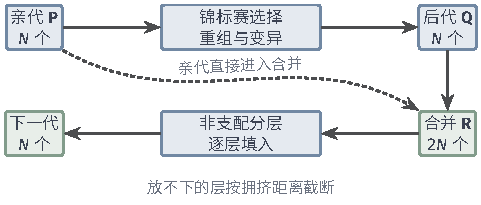
\includegraphics[width=81.5mm]{figures/05-optimization/07-multiple-criteria-and-nested-optimization/tikz/moo-nsga-flow/figure.pdf}
  \caption{NSGA-II的一代。亲代经锦标赛选择、重组与变异产生后代，亲代与后代合并成$2N$个候选，分层后逐层填入下一代，最后放不下的那一层按拥挤距离从大到小取。}
  \label{fig:moo-nsga-flow}
\end{BookInlineFigure}

\needspace{6\baselineskip}
\paragraph{变量}
\begin{itemize}
 \item 种群$\bm{P}$，$N$个候选及其目标向量，每个候选的层号与拥挤距离；
 \item 后代$\bm{Q}$，$N$个候选；合并的集合$\bm{R}=\bm{P}\cup\bm{Q}$；
 \item 分层计算中的辅助量：$S_{\bm{p}}$是$\bm{p}$支配的点集，$n_{\bm{p}}$是支配$\bm{p}$的点数。
\end{itemize}

\paragraph{初始化}
随机产生$N$个候选并评价，分层并计算拥挤距离。下面用例子说明一代中的选择。假设合并后得到八个候选，它们是式~\eqref{eq:moo-candidates}的六个点，加上
\[
 G=(3,7),\qquad H=(6,7).
\]

\needspace{6\baselineskip}
\paragraph{每轮更新}
\begin{enumerate}
 \item 产生后代：用二元锦标赛选亲代，比较时层号小者胜，层号相同时拥挤距离大者胜；再做重组和变异。例中假定后代已经产生并合并。

 \item 合并亲代和后代，对每一点计算$n_{\bm{p}}$和$S_{\bm{p}}$。例中
 \[
  n_A=n_B=n_C=n_D=0,\quad n_E=2,\quad n_F=n_G=1,\quad n_H=5.
 \]
 $E$被$B,C$支配，$F$被$D$支配，$G$被$B$支配，$H$被$B,C,D,E,G$支配。

 \item 分层：$n_{\bm{p}}=0$的点组成第一层，把它们支配的点的$n$减一，$n$减到零的点组成下一层，依此类推。例中第一层是$\{A,B,C,D\}$。把它们去掉后$n_E=n_G=n_F=0$，第二层是$\{E,F,G\}$，第三层是$\{H\}$，见图~\ref{fig:moo-nsga-layers}(a)。

 \item 逐层填入下一代，直到某一层放不下。例中取$N=6$，第一层四个点全部进入，还差两个名额。

 \item 放不下的那一层，计算拥挤距离~\eqref{eq:moo-crowding}，按从大到小取够。例中第二层$G,E,F$按$f_1$排序是$G,E,F$，$G,F$是端点，距离为无穷；$E$的距离是
 \[
  D(E)=\frac{7-3}{7-3}+\frac{7-1}{7-1}=2.
 \]
 所以取$G$和$F$，$E$被淘汰。下一代是$\{A,B,C,D,F,G\}$。
\end{enumerate}

这一例也提醒我们，$F$虽然只是弱Pareto最优点，却因为端点的身份进入了下一代。分层只反映种群内部的关系。

截断也可能发生在第一层。若$N=3$，第一层四个点要留三个。$A$和$D$是端点，距离为无穷。其余两点的距离由式~\eqref{eq:moo-crowding}算出：
\[
 D(B)=\frac{4-1}{5}+\frac{8-4}{7}\approx1.171,\qquad
 D(C)=\frac{6-2}{5}+\frac{5-1}{7}\approx1.371.
\]
所以保留$A,C,D$，淘汰$B$，图~\ref{fig:moo-nsga-layers}(b)画出了这两个长方形。$C$在加权和下永远选不上，在这里却因为不拥挤而被留下：种群搜索的比较只用支配和距离，不要求支撑。

\begin{BookInlineFigure}
  \centering
  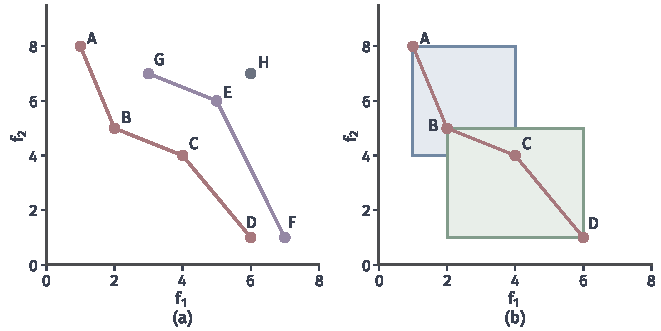
\includegraphics[width=112mm]{figures/05-optimization/07-multiple-criteria-and-nested-optimization/matplotlib/moo-nsga-layers/figure.pdf}
  \caption{八个候选的非支配排序与拥挤距离。(a)红色、紫色、灰色依次是第一、二、三层。(b)第一层内$B$与$C$的拥挤长方形，分别以$A,C$和$B,D$为角，$C$的长方形更大。}
  \label{fig:moo-nsga-layers}
\end{BookInlineFigure}

\paragraph{运行效果}
一代中比较支配关系的开销是$O(mN^2)$，拥挤距离的排序是$O(mN\log N)$，加上$N$次目标评价。目标评价昂贵时，主要开销是评价的次数。

图~\ref{fig:moo-nsga-run}是在一个五维问题上的实际运行。取$\bm{x}\in[0,1]^5$，
\begin{equation}
 f_1=x_1,\quad \gamma=1+\frac{9}{4}\sum_{j=2}^{5}x_j,\quad f_2=\gamma\Bigl(1-\bigl(f_1/\gamma\bigr)^2\Bigr).
 \label{eq:moo-zdt}
\end{equation}
当$x_2=\cdots=x_5=0$时$\gamma=1$，$f_2=1-f_1^2$，这就是式~\eqref{eq:moo-concave}的抛物线前沿。其余变量把点往上推。种群规模为$40$，运行$200$代，随机种子固定。

\begin{BookInlineFigure}
  \centering
  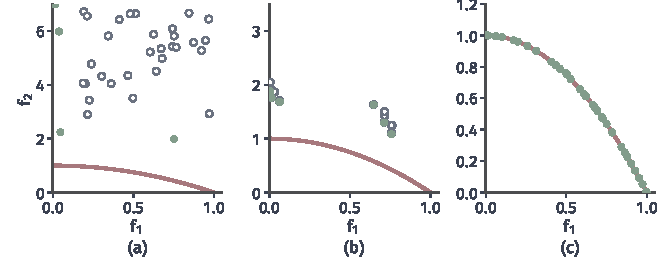
\includegraphics[width=112mm]{figures/05-optimization/07-multiple-criteria-and-nested-optimization/matplotlib/moo-nsga-run/figure.pdf}
  \caption{NSGA-II在式~\eqref{eq:moo-zdt}上的种群，种群规模$40$。红线是真实前沿，绿点是当前种群的第一层，空心点是其余个体。(a)初始种群。(b)第$10$代，第一层有$12$个点，互不支配，但离前沿还很远。(c)第$200$代，$40$个点都在前沿附近。三幅图的纵轴范围不同。}
  \label{fig:moo-nsga-run}
\end{BookInlineFigure}

第$10$代的$12$个点互不支配，却离真实前沿还很远。这正是必须记住的一点：有限种群内部互不支配，不能说明它们是Pareto最优的。算法没有全局保证，它的结果要靠第~\ref{sec:moo-front-evaluation}节的量来检查。加权和扫描在这个问题上只能得到两个端点，这里的种群搜索能把点散布到整条前沿上，这是它的优势。

\section{前沿的评价}
\label{sec:moo-front-evaluation}

算法交出了一组候选，这组候选好不好？真实前沿通常是未知的，所以要明确：在固定目标尺度和计算预算的情况下，能报告哪些可计算的量，它们分别说明什么。本节先看单个候选的质量，再看整组候选的覆盖范围。

\subsection{候选质量}
\label{sec:moo-candidate-quality}

一个候选点要检查什么？这一小节列出三项检查：是否可行，它自己的子问题解得好不好，以及是否还有共同下降的余地。

\paragraph{约束违反}
第一项是可行性。对每个候选报告最大约束违反量
\begin{equation}
 \mathrm{viol}(\bm{x})=\max\Bigl\{\max_j\,[g_j(\bm{x})]_+,\ \max_k\,\lvert h_k(\bm{x})\rvert\Bigr\},
 \label{eq:moo-violation}
\end{equation}
其中$[v]_+=\max\{v,0\}$。违反约束的点不能参与支配比较：稍微违反约束的点常常看起来更好，让它留在候选集中，会把真正可行的点错误地淘汰掉。

\paragraph{两种残差}
第二项是该候选作为优化结果的误差，这要看它是怎么得来的，要回答的问题也不同。

若候选来自权重$\bm{w}$的无约束加权和，就看它作为这个单目标问题的解有多准，用\term{标量子问题误差}（scalar subproblem error）衡量，光滑无约束时常用梯度范数
\begin{equation}
 \rho_{\bm{w}}(\bm{x})=\Bigl\lVert\sum_{i=1}^mw_i\nabla f_i(\bm{x})\Bigr\rVert_2.
 \label{eq:moo-scalar-residual}
\end{equation}

若候选是作为Pareto驻定点提交的，要看的是\term{共同下降残差}（common descent residual）$\lVert\bar{\bm{g}}(\bm{x})\rVert_2$，也就是式~\eqref{eq:moo-min-norm}中的最短长度。

这两种残差回答的问题不同。由于$\bar{\bm{g}}$是所有凸组合中最短的，对任意$\bm{w}\in\Delta_m$，
\begin{equation}
 \lVert\bar{\bm{g}}(\bm{x})\rVert_2\leq\rho_{\bm{w}}(\bm{x}).
 \label{eq:moo-residual-order}
\end{equation}
标量残差小，共同下降残差必定也小；反过来不成立。

在例~\eqref{eq:moo-iso}上算两个候选，权重都取$(1/2,1/2)$。第一个候选$\hat{\bm{x}}=(0.9,0.1)$在解集上，
\[
 \bm{g}_1=(-0.1,0.1),\qquad\bm{g}_2=(0.9,-0.9).
\]
两个梯度反向，$\lVert\bar{\bm{g}}\rVert_2=0$，它是驻定的。但
\[
 \rho_{\bm{w}}=\lVert(0.4,-0.4)\rVert_2\approx0.566.
\]
所以这个点是前沿上的一点，却不是“两项同样重要”这个偏好下的解。

第二个候选$\hat{\bm{x}}=(0.6,0.5)$略微偏离解集，
\[
 \bm{g}_1=(-0.4,0.5),\qquad\bm{g}_2=(0.6,-0.5).
\]
由式~\eqref{eq:moo-theta-two}算出$\theta^\star=0.55$，$\bar{\bm{g}}=(0.05,0.05)$，其长度约为$0.071$；而$\rho_{\bm{w}}=\lVert(0.1,0)\rVert_2=0.1$。两个残差都不为零，式~\eqref{eq:moo-residual-order}成立。

图~\ref{fig:moo-candidate-residual}把这种差别沿着整条线段画了出来：解集上共同下降残差处处为零，标量残差却只在$s=1/2$处为零。偏离解集的距离加入后，两种残差都不再为零。所以报告残差时要说清楚是哪一种。若目的是“实现这个偏好”，就看$\rho_{\bm{w}}$；若目的是“候选不能再被一阶共同改进”，就看$\lVert\bar{\bm{g}}\rVert_2$。

\begin{BookInlineFigure}
  \centering
  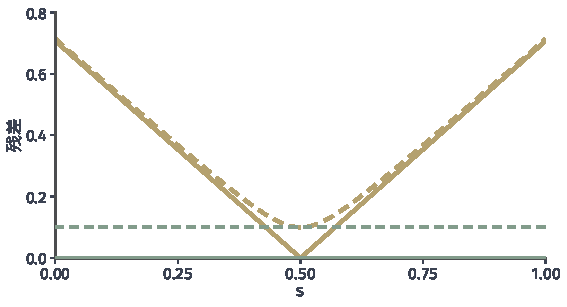
\includegraphics[width=96mm]{figures/05-optimization/07-multiple-criteria-and-nested-optimization/matplotlib/moo-candidate-residual/figure.pdf}
  \caption{例~\eqref{eq:moo-iso}中两种残差沿$\bm{x}(s)=(1-s,s)+\delta(1,1)/\sqrt2$的变化。绿线是共同下降残差，黄线是$\bm{w}=(1/2,1/2)$的标量残差，实线为$\delta=0$，虚线为$\delta=0.1$。}
  \label{fig:moo-candidate-residual}
\end{BookInlineFigure}

约束问题中，$\rho_{\bm{w}}$和$\lVert\bar{\bm{g}}\rVert_2$要换成相应的KKT残差，即式~\eqref{eq:moo-kkt}的左端在给定乘子下的范数，再加上互补松弛的误差。

\paragraph{筛选的局限}
第三项是把候选集中被支配的点剔除，用第~\ref{sec:moo-scan}节的存档方法即可。剔除之后剩下的点互不支配，但这只是在已有候选之间比较。

图~\ref{fig:moo-hidden-dominator}中，$A,B,C,D$互不支配。如果有一个没被算到的方案$\bm{P}=(3,3)$，它支配$C$，粉色区域中的方案都比它差。有限候选之间的筛选，永远不能证明不存在尚未找到的支配方案。

\begin{BookInlineFigure}
  \centering
  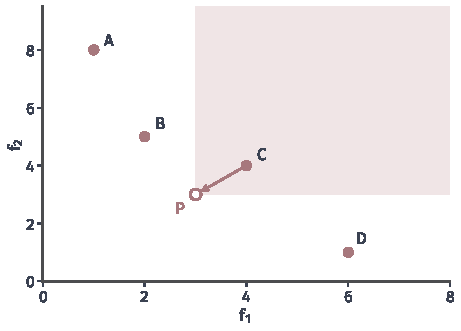
\includegraphics[width=78mm]{figures/05-optimization/07-multiple-criteria-and-nested-optimization/matplotlib/moo-hidden-dominator/figure.pdf}
  \caption{有限候选的筛选不足以判定最优。红点$A,B,C,D$互不支配，尚未找到的方案$\bm{P}=(3,3)$（红色空心点）却支配$C$，$C$落在$\bm{P}$的被支配区域（粉色）中。}
  \label{fig:moo-hidden-dominator}
\end{BookInlineFigure}

证明一个候选是全局Pareto最优的办法有两种：问题是凸的，用定理~\ref{thm:moo-kkt-sufficient}；或者全局求解一个能够选中它的标量子问题。两种都不能依靠候选之间的比较。

\subsection{覆盖范围}
\label{sec:moo-coverage}

单个候选合格，整组未必合格，它们可能都挤在前沿的一小段上。这一小节讨论怎样用数字描述整组候选的质量，以及每个数字的局限。

\paragraph{超体积}
取一个比所有候选都差的\term{参考点}$\bm{r}$，也就是各分量都大于候选相应分量的点。候选集$\bm{S}$支配的、并被$\bm{r}$界住的区域的体积称为\term{超体积}（hypervolume）：
\begin{equation}
 \mathrm{HV}(\bm{S};\bm{r})=\mathrm{vol}\Bigl(\bigcup_{\bm{y}\in\bm{S}}\{\bm{z}:\bm{y}\leq\bm{z}\leq\bm{r}\}\Bigr).
 \label{eq:moo-hv}
\end{equation}
一个指标把“离前沿多近”和“覆盖多宽”都包含进来：候选越靠前沿，被支配区域越大；候选越分散，并集越大。

两个目标时超体积可以按条带求和。把候选按$f_1$从小到大排序，设互不支配，记第$i$点为$(y_{1,i},y_{2,i})$，$i=1,\ldots,N$，并约定$y_{1,N+1}=r_1$。则
\begin{equation}
 \mathrm{HV}=\sum_{i=1}^{N}(y_{1,i+1}-y_{1,i})(r_2-y_{2,i}).
 \label{eq:moo-hv-2d}
\end{equation}

对$A,B,C,D$取$\bm{r}=(8,9)$，四个条带的面积是
\[
 (2-1)(9-8)=1,\quad(4-2)(9-5)=8,\quad(6-4)(9-4)=10,\quad(8-6)(9-1)=16,
\]
总和$\mathrm{HV}=35$，见图~\ref{fig:moo-hypervolume}。把$E$或$F$加进来，超体积不变，因为它们支配的区域已经被覆盖。把$C$去掉，超体积变成$33$，$C$独占的贡献是$(6-4)(5-4)=2$。

\begin{BookInlineFigure}
  \centering
  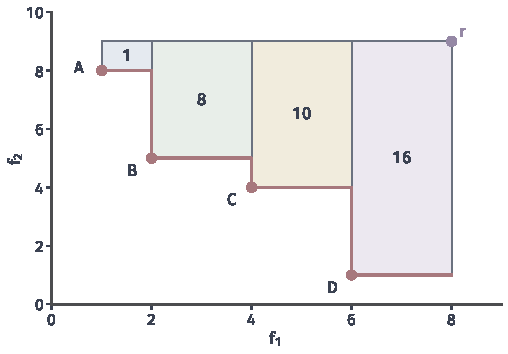
\includegraphics[width=86mm]{figures/05-optimization/07-multiple-criteria-and-nested-optimization/matplotlib/moo-hypervolume/figure.pdf}
  \caption{$A,B,C,D$的超体积，参考点$\bm{r}=(8,9)$。彩色条带的面积分别是$1,8,10,16$，合计$35$。红色阶梯线是这组候选支配区域的左下边界。}
  \label{fig:moo-hypervolume}
\end{BookInlineFigure}

超体积的好处在于它和支配关系是相容的。

\begin{theorem}[超体积的单调性]
\label{thm:moo-hv-monotone}
设$\bm{S},\bm{S}'$的所有点都逐分量不大于$\bm{r}$。若对每个$\bm{y}'\in\bm{S}'$，存在$\bm{y}\in\bm{S}$使$\bm{y}\leq\bm{y}'$，则
\begin{equation}
 \mathrm{HV}(\bm{S};\bm{r})\geq\mathrm{HV}(\bm{S}';\bm{r}).
 \label{eq:moo-hv-monotone}
\end{equation}
\end{theorem}

\begin{proof}
若$\bm{y}\leq\bm{y}'\leq\bm{z}\leq\bm{r}$，则$\bm{y}\leq\bm{z}\leq\bm{r}$。所以$\bm{S}'$对应的并集包含在$\bm{S}$对应的并集中，体积不减。
\end{proof}

也就是说，把一组候选换成支配它们的另一组，超体积不会下降。

\paragraph{参考点和尺度}
超体积不是一个自足的数字，它依赖参考点。设$\bm{S}_1=\{(1,6),(6,1)\}$，$\bm{S}_2=\{(3,3)\}$。取$\bm{r}=(7,7)$，由式~\eqref{eq:moo-hv-2d}，
\[
 \mathrm{HV}(\bm{S}_1)=5\times1+1\times6=11,\qquad\mathrm{HV}(\bm{S}_2)=4\times4=16.
\]
$\bm{S}_2$更好。取$\bm{r}=(20,20)$，
\[
 \mathrm{HV}(\bm{S}_1)=5\times14+14\times19=336,\qquad\mathrm{HV}(\bm{S}_2)=17\times17=289.
\]
$\bm{S}_1$更好。参考点越远，越看重前沿的两端，见图~\ref{fig:moo-hv-reference}。比较不同算法时，参考点必须事先固定，并且和结果一起报告。

\begin{BookInlineFigure}
  \centering
  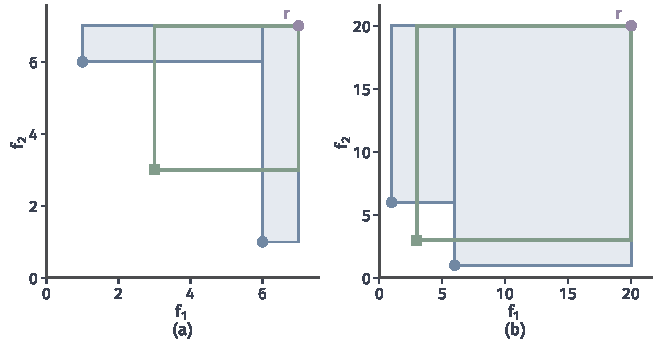
\includegraphics[width=112mm]{figures/05-optimization/07-multiple-criteria-and-nested-optimization/matplotlib/moo-hv-reference/figure.pdf}
  \caption{超体积比较依赖参考点。蓝色区域属于$\bm{S}_1=\{(1,6),(6,1)\}$，绿色方框属于$\bm{S}_2=\{(3,3)\}$。(a)$\bm{r}=(7,7)$，$\bm{S}_2$较大。(b)$\bm{r}=(20,20)$，$\bm{S}_1$较大。}
  \label{fig:moo-hv-reference}
\end{BookInlineFigure}

尺度的影响也要说明。把目标$k$乘以$c>0$，参考点相应乘以$c$，所有超体积同乘$c$，比较结果不变。但把目标归一化时，若参考范围随候选集而变，每组候选用的就是不同的尺子，比较便失去了共同的基准。

\paragraph{空缺与取舍范围}
超体积把很多信息压成一个数，可能掩盖分布上的差别。还要报告相邻候选之间的最大间距和目标的取舍范围。

在例~\eqref{eq:moo-iso}的前沿上，用$s$值表示候选，取$\bm{S}_1:\ s=0.1,0.5,0.9$与$\bm{S}_2:\ s=0.24,0.515,0.975$。取$\bm{r}=(1.2,1.2)$，两者的超体积都等于$1.0897$，见图~\ref{fig:moo-coverage-distance}。可是把前沿两端也算上，$\bm{S}_1$的最大相邻间距约为$0.609$，$\bm{S}_2$约为$0.724$，$\bm{S}_2$在靠$f_2$轴的一端空出了更大的一段。

\begin{BookInlineFigure}
  \centering
  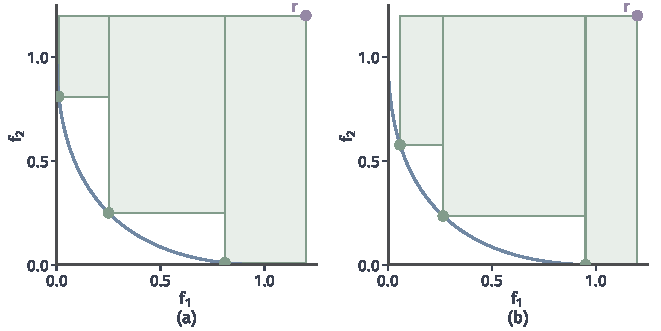
\includegraphics[width=112mm]{figures/05-optimization/07-multiple-criteria-and-nested-optimization/matplotlib/moo-coverage-distance/figure.pdf}
  \caption{两组超体积相同（$\bm{r}=(1.2,1.2)$，$\mathrm{HV}=1.0897$）的候选，蓝线是真实前沿。(a)$s=0.1,0.5,0.9$。(b)$s=0.24,0.515,0.975$，最大相邻间距更大。}
  \label{fig:moo-coverage-distance}
\end{BookInlineFigure}

\paragraph{到参考前沿的距离}
若有可信的参考前沿$\bm{R}$，比如问题有解析解，或者是长时间计算汇总的结果，可以进一步计算候选集与它的距离。两个常用的量是\term{世代距离}（generational distance，GD）和\term{反向世代距离}（inverted generational distance，IGD）：
\begin{equation}
 \begin{aligned}
  \mathrm{GD}&=\frac{1}{\lvert\bm{S}\rvert}\sum_{\bm{y}\in\bm{S}}\min_{\bm{p}\in\bm{R}}\lVert\bm{y}-\bm{p}\rVert_2,\\
  \mathrm{IGD}&=\frac{1}{\lvert\bm{R}\rvert}\sum_{\bm{p}\in\bm{R}}\min_{\bm{y}\in\bm{S}}\lVert\bm{y}-\bm{p}\rVert_2.
 \end{aligned}
 \label{eq:moo-gd-igd}
\end{equation}

GD看候选离前沿有多近，IGD看前沿被候选覆盖得多好。图~\ref{fig:moo-coverage-distance}的两组候选都在前沿上，GD都是零。IGD用$1001$个参考点计算，$\bm{S}_1$约为$0.143$，$\bm{S}_2$约为$0.163$，这里区分出了两组候选的覆盖差别。

这些量都要有参考前沿才能算。若参考前沿是其他算法的结果，算出的就只是相对的差别，不是真实误差。

\paragraph{多个指标一起看}
图~\ref{fig:moo-nsga-indicators}是图~\ref{fig:moo-nsga-run}那次运行的指标曲线，参考点取$\bm{r}=(1.1,1.1)$。超体积在第$40$代已经到$0.512$，真实前沿对应的值是$0.5433$，第$200$代是$0.5245$。到参考前沿的平均距离第$100$代约为$0.0141$，第$200$代约为$0.0153$，并不单调。

\begin{BookInlineFigure}
  \centering
  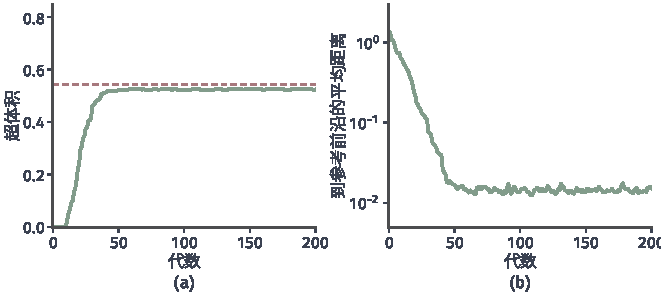
\includegraphics[width=112mm]{figures/05-optimization/07-multiple-criteria-and-nested-optimization/matplotlib/moo-nsga-indicators/figure.pdf}
  \caption{NSGA-II运行中的指标，问题为式~\eqref{eq:moo-zdt}。(a)超体积，$\bm{r}=(1.1,1.1)$，红色虚线是真实前沿的值$0.5433$。(b)种群第一层到参考前沿的IGD，纵轴为对数。曲线后段不是单调的。}
  \label{fig:moo-nsga-indicators}
\end{BookInlineFigure}

种群只有$40$个点，覆盖不了整条曲线，超体积不会达到$0.5433$，这个差额来自有限的点数。同一种群的第一层不断变化时，IGD也可以上下波动。不能用一个集合指标代替所有判断。表~\ref{tab:moo-indicators}列出各个量各自回答的问题。

\begin{BookInlineTable}
  \centering
  \caption{候选集的常用评价量。}
  \label{tab:moo-indicators}
  \begin{tabular}{@{}lll@{}}
    \toprule
    量 & 回答的问题 & 需要的条件\\
    \midrule
    约束违反 & 是否可行 & 约束函数\\
    标量残差 & 这次偏好解得准不准 & 权重或阈值\\
    共同下降残差 & 还能否一阶共同改进 & 梯度\\
    超体积 & 支配区域多大 & 固定的$\bm{r}$与尺度\\
    最大间距 & 前沿上有无大空缺 & 目标尺度\\
    GD与IGD & 离参考前沿多近 & 可信的参考前沿\\
    \bottomrule
  \end{tabular}
\end{BookInlineTable}

把这些量都算出来，能说的话仍然有限：这组候选满足约束，单点的残差如此，在这个参考点下超体积如此。不能说“已经恢复了完整的Pareto前沿”，除非另有理论保证。

\section{本章小结}
\label{sec:moo-summary}

本章从“两个目标各有所长的方案谁更好”出发。结论是，不依赖偏好的比较只有支配关系，由它得到的是一组互不支配的方案，而不是一个方案。目标冲突不会因为单目标算法更强而消失，强的算法只能更快地解出某一个偏好下的问题。

支配关系是第一层判断，它不受单位影响。权重、距离和归一化都依赖尺度，使用时要写明单位与参考范围。

偏好由三种标量化表达。加权和相当于定价，权重全正的全局解是Pareto最优的，凸问题中非负权重足以选中每个弱Pareto最优点，但在非凸前沿上会遗漏非支撑点。阈值约束相当于定预算，加权Chebyshev相当于要求各项接近某个水平，二者不需要凸性就能选中每个Pareto点，但可能返回并列的弱Pareto最优解，需要第二阶段的择优。

局部信息给出一阶判别。Pareto驻定说明不存在严格共同下降的方向，这是局部弱Pareto最优的必要条件，有约束时要在约束资格下配合乘子；要由它推出全局结论，还需要凸性，权重全正时才能得到Pareto最优。多梯度下降从梯度凸包的最小范数元得到共同下降方向，配合共同步长使每个目标都下降，一次运行收敛到一个驻定点。

要得到一组候选，可以扫描偏好参数，用热启动降低代价，按空缺补点，并用非支配存档保存结果；也可以用NSGA-II这样的群体搜索，以分层和拥挤距离代替单目标的排序。两者都要在固定的目标尺度下，用约束违反、残差、超体积、间距以及到参考前沿的距离来检查。

图~\ref{fig:moo-summary}汇总了四种结果之间的关系。加权最优、Pareto驻定、全局Pareto最优和有限候选集的覆盖是四种不同的结论，从一种到另一种都需要说明所依赖的条件。

\begin{BookInlineFigure}
  \centering
  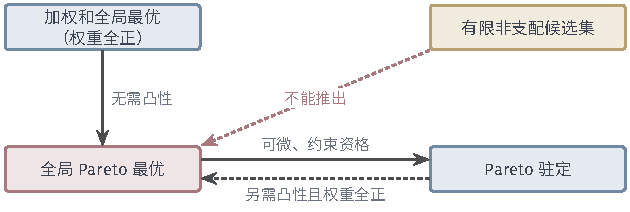
\includegraphics[width=106.7mm]{figures/05-optimization/07-multiple-criteria-and-nested-optimization/tikz/moo-summary/figure.pdf}
  \caption{四种结果的关系。实线箭头在标注的条件下成立，虚线箭头需要额外的条件，红色虚线表示有限候选集互不支配不能推出全局Pareto最优。}
  \label{fig:moo-summary}
\end{BookInlineFigure}

